\documentclass[aspectratio=169, 9pt]{beamer}
\usepackage{caption}
\usepackage{subcaption}
\usepackage{braket}
%
\usepackage{amsmath}
%%%%%%%%%%%%%%%%%%%
\newcommand{\Eins}{\mathds{1}}

\normalem
\usepackage{tikz}

\def\clap#1{\hbox to 0pt{\hss#1\hss}}
\def\mathllap{\mathpalette\mathllapinternal}
\def\mathrlap{\mathpalette\mathrlapinternal}
\def\mathclap{\mathpalette\mathclapinternal}
\def\mathllapinternal#1#2{%
\llap{$\mathsurround=0pt#1{#2}$}}
\def\mathrlapinternal#1#2{%
\rlap{$\mathsurround=0pt#1{#2}$}}
\def\mathclapinternal#1#2{%
\clap{$\mathsurround=0pt#1{#2}$}}


\newcommand{\bc}{\begin{center}}
\newcommand{\ec}{\end{center}}
\def\t0{t\text{$=$}0}
\def\ix0{\xi\text{$=$}0}
%\def\wg{\stackrel{\text{\scriptsize{worm}}}{\text{\scriptsize{gear}}}}
\def\wg{{g_{1T}}}

\newcommand{\bea}{\vspace{-0mm}\begin{eqnarray}}
\newcommand{\eea}{\end{eqnarray}}
\newcommand{\Dlr}{{D^{\hspace{-0.8em}%
      \raisebox{0.8ex}{$\scriptstyle\leftrightarrow$}}}{}}
\newcommand{\Dl}{{D^{\hspace{-0.8em}%
      \raisebox{0.8ex}{$\scriptstyle\leftarrow$}}}{}}
\newcommand{\Dr}{{D^{\hspace{-0.8em}%
      \raisebox{0.8ex}{$\scriptstyle\rightarrow$}}}{}}
%
\newcommand{\gev}{\operatorname{GeV}}
\newcommand{\mev}{\operatorname{MeV}}
\newcommand{\fm}{\operatorname{fm}}
\usepackage{graphicx}
\usepackage{subcaption}
\newcommand{\ms}{\mskip 1.5mu}

\newcommand{\toolkit}[1]{{\tt #1}}

% editing markup, old version:
%\newcommand{\todo}[1]{$\langle$\textbf{TODO:} \emph{#1}$\rangle$}
%\newcommand{\muline}[1]{\uline{#1}}
%\newcommand{\mxout}[1]{\xout{#1}}
%\newcommand{\bnew}{$\langle$\textbf{new:}$\rangle$}
%\newcommand{\enew}{$\langle$\textbf{endnew}$\rangle$}
%\newcommand{\red}[1]{\textcolor{red}{[ #1 ]}}

% editing markup:
\newcommand{\TD}[1]{$\langle$\textbf{TODO:} \emph{#1}$\rangle$}
\newcommand{\todo}[1]{$\langle$\textbf{TODO:} \emph{#1}$\rangle$}
\newcommand{\muline}[1]{{\color{red!50!black}{#1}}}
\newcommand{\mxout}[1]{{\color{black!20!white}{#1}}}
\newcommand{\bnew}{$\langle$\textbf{new:}$\rangle$}
\newcommand{\enew}{$\langle$\textbf{endnew}$\rangle$}
\newcommand{\editnote}[1]{\marginpar{{\color{green!50!black}{#1}}}}


% editing markup deactivated:
%\newcommand{\todo}[1]{}
%\newcommand{\muline}[1]{#1}
%\newcommand{\mxout}[1]{}
%\newcommand{\bnew}{}
%\newcommand{\enew}{}

\newcommand{\units}[1]{\ensuremath{\,\mathrm{#1}}}
\newcommand{\braKet}[3]{#3\langle#1#3|#2#3\rangle}
\newcommand{\Tr}{\mathrm{tr}}
\newcommand{\BTr}{\mathrm{Tr}}
\newcommand{\elll}{{\color{red}l}}
\newcommand{\latcfn}{\ensuremath{C}}
\usepackage{graphicx}
\newcommand{\tpm}{\ensuremath{{\,\pm\,}}}

\newcommand{\prp}{\perp}
\newcommand{\transp}{\mathsf{T}}
\newcommand{\GammaOp}{\Gamma}
\newcommand{\GammaDist}{\ensuremath{\Gamma^\text{d}}}
\newcommand{\GammaTwo}{\ensuremath{\Gamma^\text{2pt}}}
\newcommand{\GammaThr}{\ensuremath{\Gamma^\text{3pt}}}
\newcommand{\GammaDiq}{\ensuremath{\Gamma^\text{diq}}}
\newcommand{\lat}{{\text{lat}}}
\newcommand{\ren}{{\text{ren}}}
\newcommand{\unren}{{\text{unren}}}
\newcommand{\norm}{{\text{norm}}}
\newcommand{\tcdot}{{\cdot}}
\newcommand{\ldotP}{{\elll\!\cdot\!P}}

\newcommand{\myRe}{\ensuremath{\mathrm{Re}}}
\newcommand{\myIm}{\ensuremath{\mathrm{Im}}}

\newcommand{\dlangle}{{\rlap{\big\langle}\hskip 0.1em\big\langle}}
\newcommand{\drangle}{{\rlap{\big\rangle}\hskip 0.1em\big\rangle}}

\newcommand{\Wline}[1]{\ensuremath{{\mathcal{U}}[#1]}}
\newcommand{\WlineC}[1]{\ensuremath{{\mathcal{U}}{[#1]}}}
\newcommand{\WlineClat}[1]{\ensuremath{{\mathcal{U}}^\text{lat}{[#1]}}}
\newcommand{\WlineI}[2]{\ensuremath{{\mathcal{U}}#1{[#2]}}}
\newcommand{\Wlineren}[1]{\ensuremath{{\mathcal{U}}^\text{ren}[#1]}}

\newcommand{\mean}[1]{\ensuremath{\left\langle{#1}\right\rangle}}
\newcommand{\vect}[1]{\ensuremath{\boldsymbol{#1}}}
\newcommand{\vprp}[1]{\vect{#1}_{\mathrm T}}

\newcommand{\mmin}{{\text{min}}}

\newcommand{\quark}{q}
\newcommand{\nucl}[1]{{#1}}
\newcommand{\Quark}{Q}
\newcommand{\Afield}{A}

\newcommand{\MDM}{\mathcal{M}}
\newcommand{\tMDM}{\tilde{\mathcal{M}}}
\newcommand{\tAmp}{\widetilde{A}}
\newcommand{\tBmp}{\widetilde{B}}
\newcommand{\TFM}{{\hat{\mathbb{T}}}}
\newcommand{\renZ}{Z}

%\newcommand{\len}{\mathcal{L}}
\newcommand{\len}{\ell}

\newcommand{\nplus}{\ensuremath{\bar n}}
\newcommand{\nminus}{\ensuremath{n}}


\newcommand{\TMD}{TMD\xspace}
\newcommand{\TMDs}{TMDs\xspace}

\newcommand{\sW}{\ensuremath{\text{sW}}}

\newcommand{\toddmark}[1]{\ensuremath{\Bigg[#1\Bigg]_{\text{\tiny{odd}}}}}
\newcommand{\Eu}[1]{#1}

\newcommand{\fourint}{\ensuremath{\int_\mathcal{F}}}
\newcommand{\xfourint}{\ensuremath{\int_\mathcal{M}}}


\newcommand{\conherm}{\ensuremath{(\dagger)}}
\newcommand{\conpar}{\ensuremath{(\mathrm{P})}}
\newcommand{\contime}{\ensuremath{(\mathrm{T})}}
\newcommand{\myeps}{\ensuremath{\epsilon}}

\newcommand{\xmom}[1]{{\ensuremath{[#1]}}}
\newcommand{\ktmom}[1]{{\ensuremath{(#1)}}}
\newcommand{\xktmom}[2]{{\xmom{#1}\ktmom{#2}}}

\newcommand{\bvec}{b}
\newcommand{\softf}{\mathcal{S}}
\newcommand{\mN}{m_N}
\newcommand{\nf}{n_f}


\newcommand{\sgn}{\mathrm{sgn}}
\newcommand{\nbdash}{\protect\nobreakdash-\hspace{0pt}}

\newcounter{fnnumber}
\newcounter{fnnumberamp}
\newcommand{\MSbar}{\overline{\text{MS}}}

\newcommand{\kei}{k}

\newcommand{\unsub}{\text{unsubtr.}}
\newcommand{\zetahat}{{\hat \zeta}}

%%%%%%%%%%%%%%%%%%%
% Choose how your presentation looks.
%
% For more themes, color themes and font themes, see:
% http://deic.uab.es/~iblanes/beamer_gallery/index_by_theme.html
%
\mode<presentation>
{
  \usetheme{Boadilla}      % or try Darmstadt, Madrid, Warsaw, ...
  \usecolortheme{default} % or try albatross, beaver, crane, ...
  \usefonttheme{serif}  % or try serif, structurebold, ...
  \setbeamertemplate{navigation symbols}{}
  \setbeamertemplate{caption}[numbered]
} 

\usepackage[english]{babel}
\usepackage[utf8]{inputenc}
\usepackage[T1]{fontenc}

\title[Lattice QCD calculations of TMDs]{\textbf{Lattice QCD calculations of \\
Transverse Momentum Dependent \\
Parton
Distribution Functions (TMDs)}}
\author[hari1729@nmsu.edu] % (optional, for multiple authors)
{\textbf{Hariprashad Ravikumar}\inst{$\dagger$}\\~\\
 Doctoral Advisor\\
 \textbf{Dr. Michael Engelhardt}\inst{$\dagger$}\\
 $~$\\
 Doctoral Committee\\
 \textbf{Dr. Matthew Sievert}\inst{$\dagger$},  \textbf{Dr. Vassili Papavassiliou}\inst{$\dagger$},  \textbf{Dr. Tuan Le}\inst{$\dagger$}\\}

\institute[] % (optional)
{
  \inst{$\dagger$}%
  New Mexico State University, USA
}
\date[]{Nov 09, 2023}

\begin{document}
\begin{frame}
  \titlepage
  \begin{figure}  [h!]
	\centering
	
\includegraphics[scale=0.13]{NMSU_BBStF-Left.eps}
	%\label{fig_nitjlogo2}
\end{figure}
\end{frame}

% Uncomment these lines for an automatically generated outline.
 %\begin{frame}{Outline}
 %  \tableofcontents
 %\end{frame}

\begin{frame}{Quarks $\&$ Gluons}
    \textbf{Hadrons are made of more fundamental particles, named "Quarks".}
    \begin{figure}
        \centering
        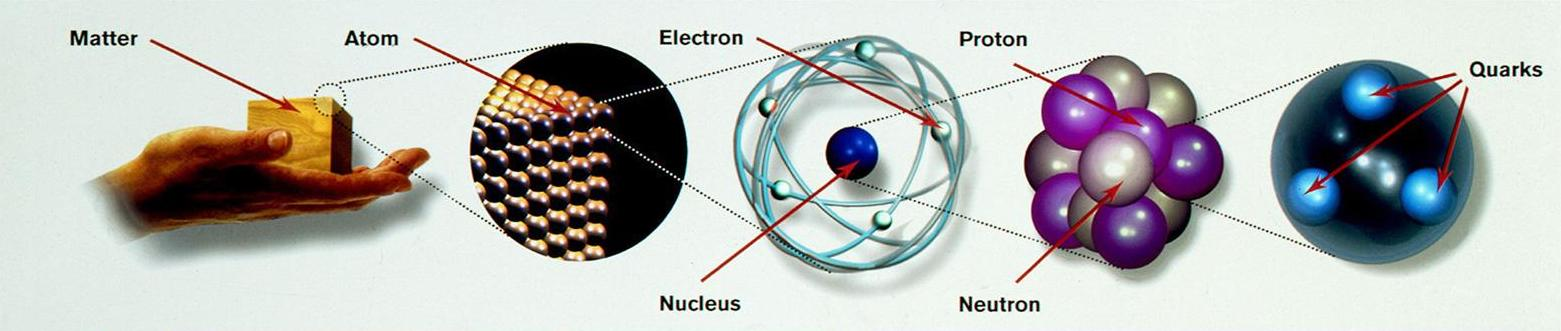
\includegraphics[scale=0.21]{cmscern.jpeg}
        \caption{All known atoms are made of electrons and quarks (credit: CMS-CERN)}
        \label{fig:enter-label}
    \end{figure}
    \begin{figure}
        \centering
        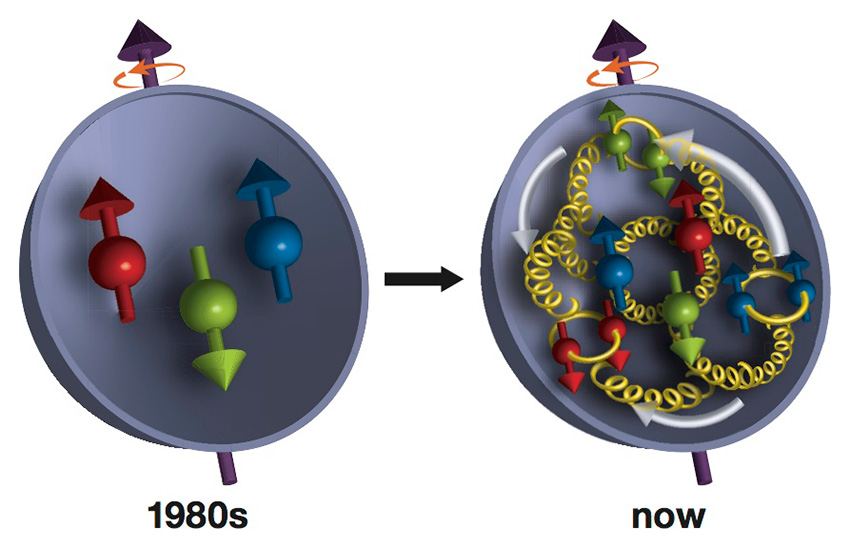
\includegraphics[scale=0.18]{nucleon-large.jpg}
        \caption{Internal structure of Hadrons [Quarks $\&$ Gluons]  (credit: BNL)}
        \label{fig:enter-label}
    \end{figure}
\end{frame}

\begin{frame}{QCD (Quantum ChromoDynamics)}
    As a quantum field theory, the QCD Lagrange density is constructed from 2 types of particle fields:
    \begin{itemize}
        \item Spin-$\frac{1}{2}$ Dirac fields (quarks): $\boxed{\psi^{i}_{f}}$
        \begin{itemize}
            \item color $i = 1, 2, 3 =N_{c}$ 
            \item flavor $f=u,d,s,c,b,t$
        \end{itemize}
        \item Massless spin-$1$ vector fields (gluons): $\boxed{A_{\mu}^{a} }$\begin{itemize}
            \item color $a=1,2,\cdots,8=N_{c}^{2}-1$, with $SU(3)$ local color gauge symmetry
        \end{itemize} 
    \end{itemize}
    \begin{align}
        \boxed{\mathcal{L}_{QCD}(\psi_{f},A_{\mu})=-\frac{1}{4}F^{2}_{\mu\nu,a}[A]+\sum_{f}\Bar{\psi}_{f}(iD_{\mu}[A]\gamma^{\mu}-m_{f})\psi_{f}}~.
    \end{align}
    
Here,
\begin{itemize}
\begin{itemize}
    \item the gluon field strength  $\boxed{F_{\mu\nu,a}[A]=\partial_{\mu}A_{\nu,a}-\partial_{\nu}A_{\mu,a}-gf_{abc}A_{\mu,b}A_{\nu,c}}$
    \item the covariant derivative $\boxed{D_{\mu}[A]=\partial_{\mu}+igA_{\mu,a}t_{a}}$
    \item the generator $t_{a}$ and structure constant $f_{abc}$ define the $SU(3)$ color algebra: $\boxed{[t_{a},t_{b}]=if_{abc}t_{c}}$
    \item $g$ is the strong coupling constant.
\end{itemize}
\end{itemize}
\end{frame}

\begin{frame}{Lattice QCD\footnote{K. G. Wilson, Confinement of Quarks, Phys. Rev. D10 (1974) 2445.}}
    $\Lambda_{4}=\{n_{\mu}=(n_{1},n_{2},n_{3},n_{4})|n_{i}\in a[0,1,\cdots,L_{i}-1]\}$ \\

\begin{align}
    \boxed{S_{gauge}=\frac{2}{g^2}\sum_{x\in{\Lambda_{4}}}\sum_{\mu<\nu}(1-Re~Tr~[P_{\mu\nu}(x)])}
\end{align}
\begin{center}
\begin{tikzpicture}[scale=1.051]
  % Define lattice points in red
  \foreach \x in {0, 1, 2, 3}
    \foreach \y in {0, 1, 2, 3}
      \fill[red] (\x, \y) circle (0.1);
\draw[|<->|, gray] (0.1, 0.1) -- (0.9, 0.1);
\node at (0.5, 0.2) {\textcolor{gray}{$a$}};
  % Draw links
  \foreach \x in {0, 1, 2, 3}
    \foreach \y in {0, 1, 2}
      \draw (\x, \y) -- (\x, \y + 1);
  \foreach \x in {0, 1, 2}
    \foreach \y in {0, 1, 2, 3}
      \draw (\x, \y) -- (\x + 1, \y);
 \draw[thick, blue] (1, 1) -- (2, 1) -- (2, 2) -- (1, 2) -- cycle;
 \draw[->, red, dashed] (1, 1) -- (0.65, 0.85);
   \node at (0.5, 0.8) {\textcolor{red}{$x$}};
  % Add labels
  \node at (1.5, 1.5) {$P_{\mu\nu}(x)$};
  % Add x and y axes
  \draw[->] (0, 0) -- (3.5, 0) node[right] {$\mu$};
  \draw[->] (0, 0) -- (0, 3.5) node[above] {$\nu$};
  % Zoom effect
  \draw[magenta, dashed] (1.5, 1.5) circle (0.8);
  \draw[->, magenta, dashed] (2.3, 1.5) -- (5.7, 1.5)
  \draw[thick, blue] (3, 2) -- (3, 3)
  \draw[blue,->, line width=1.5pt] (3, 2.5) -- ++(0,0.1);
   \node at (4.5, 2.5) {\textcolor{blue}{$U_{\nu}(y)=e^{iaA_{\nu}(y)}$}};
   \draw[->, red, dashed] (3, 2) -- (2.6, 2.2)
   \node at (2.5, 2.2) {\textcolor{red}{$y$}};
  % Create a scope for the plaquette on the left side
  \begin{scope}[xshift=6cm]
   \foreach \x in {1, 2}
    \foreach \y in {1, 2}
      \fill[red] (\x, \y) circle (0.1);
    % Create a plaquette
    \draw[magenta, dashed] (1.8, 1.5) ellipse (1.99 and 1.3);
   \draw[thick, blue] (1, 1) -- (2, 1) -- (2, 2) -- (1, 2) -- cycle;
   \draw[blue,->, line width=1.5pt] (1.5, 1) -- ++(0.1,0);
   \draw[blue,<-, line width=1.5pt] (1.5, 2) -- ++(0.1,0);
   \draw[blue,->, line width=1.5pt] (2, 1.5) -- ++(0,0.1);
   \draw[blue,<-, line width=1.5pt] (1, 1.5) -- ++(0,0.1);
   \draw[->, red, dashed] (1, 1) -- (0.65, 0.85)
   \node at (0.5, 0.8) {\textcolor{red}{$x$}};
    % Add a label for the plaquette on the left side
    \node at (1.5, 0.7) {$U_{\mu}(x)$};
    \node at (3, 1.5) {$U_{\nu}(x+\hat{\mu})$};
    \node at (1.5, 2.4) {$U^{\dagger}_{\mu}(x+\hat{\nu})$};
    \node at (0.4, 1.5) {$U^{\dagger}_{\nu}(x)$};
  \end{scope}
\end{tikzpicture}
\end{center}
where the elementary plaquette, $\boxed{P_{\mu\nu}(x)=U_{\mu}(x)U_{\nu}(x+\hat{\mu})U^{\dagger}_{\mu}(x+\hat{\nu})U^{\dagger}_{\nu}(x)}$.
\end{frame}

\begin{frame}{Lattice QCD}
    \begin{align*}
             \boxed{S_{gauge}=\frac{2}{g^2}\sum_{x\in{\Lambda_{4}}}\sum_{\mu<\nu}(1-Re~Tr~[P_{\mu\nu}(x)])=\frac{a^4}{2g^2}\sum_{x\in{\Lambda_{4}}}\sum_{\mu<\nu}tr~[F_{\mu\nu}(x)^2]+\mathcal{O}(a^2)}.
    \end{align*}
    Physical observables $\mathcal{O}$ are evaluated as an expectation value over the relevant degrees of freedom
    \begin{align}
        \boxed{\langle \mathcal{O} \rangle =\frac{\int \mathcal{D}[U]\textcolor{blue}{\mathcal{D}[\psi]\mathcal{D}[\Bar{\psi}}]~\mathcal{O}~e^{-[S_{gauge}+\textcolor{blue}{\int dx \Bar{\psi}\mathcal{M}\psi}]}}{\int\mathcal{D}[U]\textcolor{blue}{\mathcal{D}[\psi]\mathcal{D}[\Bar{\psi}]}e^{-[S_{gauge}+\textcolor{blue}{\int dx \Bar{\psi}\mathcal{M}\psi}]}}}.
    \end{align}
    The quark fields $\psi~\&~\Bar{\psi}$ are Grassmann variables:
    \begin{align}
        \boxed{\langle \mathcal{O} \rangle =\frac{\int \mathcal{D}[U]~\widetilde{\mathcal{O}}~\textcolor{blue}{det \mathcal{M}^2}e^{-[S_{gauge}]}}{\int\mathcal{D}[U]\textcolor{blue}{det \mathcal{M}^2}e^{-[S_{gauge}]}}}.
    \end{align}
    This integration results in the “contraction” of fermion–anti-fermion pairs in all possible ways (Wick's theorem), replacing them with quark propagators \textcolor{blue}{$\mathcal{M}^{-1}$}.
\end{frame}

\begin{frame}{Numerical simulation for Lattice QCD}
    The vacuum expectation value of an observable in a Monte Carlo simulation approximation: (Sum over $U_{n}$ with probability  $\propto e^{-S[U_{n}]}$)
    \begin{align*}
        \boxed{\langle O \rangle =\frac{\int \mathcal{D}[U]e^{-S_{G}[U]}O[U]}{\int\mathcal{D}[U]e^{-S_{G}[U]}}}\rightarrow\boxed{ \langle O \rangle \approx \frac{1}{N}\sum_{U_{n}}O[U_{n}]}
    \end{align*}
    \begin{figure}
        \centering
        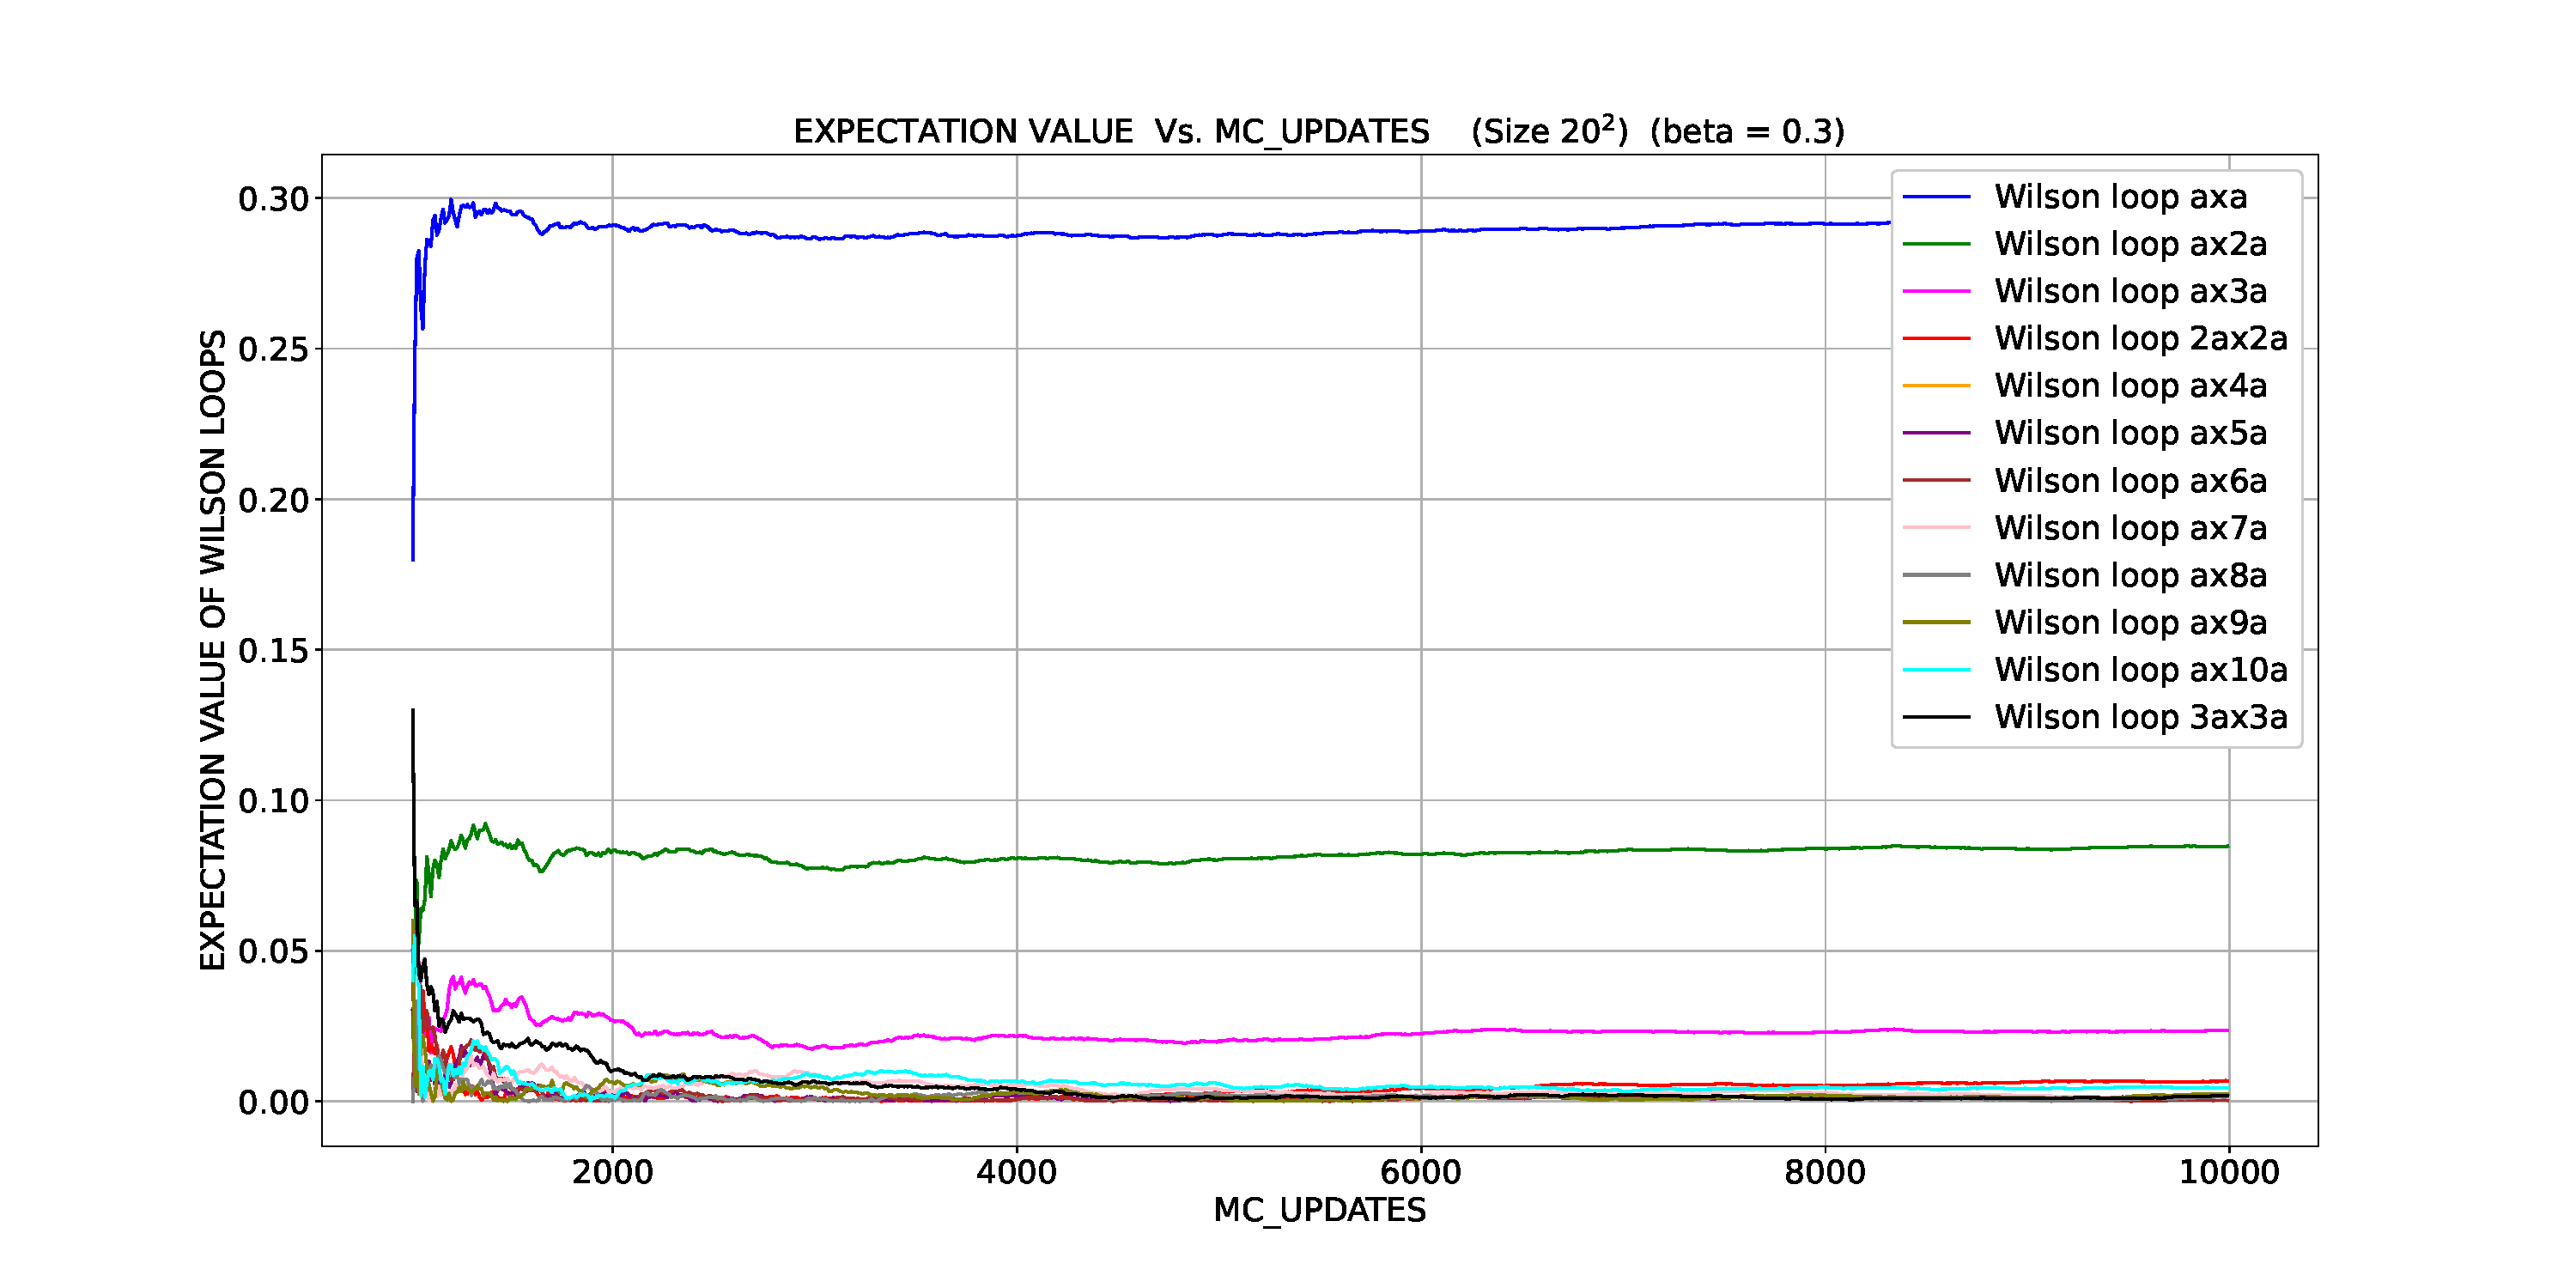
\includegraphics[scale=0.225]{mcstepsz2.pdf}
        \caption{Markov chain - Monte Carlo simulations of $\mathbb{Z}_2$ lattice gauge theory $(1+1)$ }
        \label{fig:enter-label}
    \end{figure}

\end{frame}


\begin{frame}{$SU(3)$ Wilson Loops $\&$ Quark String Tension}
    We calculated various sizes of Wilson loops $\langle W(r,t)\rangle$ and formed  Creutz\footnote{Creutz, M., Phys. Rev. Lett. 45, 313.} ratios $\chi(r,t)$ to extract quark string tension $\sigma$
    \begin{align*}
        \boxed{\chi(r,t)=-\ln{\left(\frac{\langle W(r,t)\rangle\langle W(r-1,t-1)\rangle}{\langle W(r,t-1)\langle W(r-1,t)\rangle}\right)}}\rightarrow\boxed{\chi_{\text{(t-plateau)}}(r)=\frac{A}{\hat{r}(\hat{r}+1)}+a^2\sigma}
    \end{align*}
       \begin{figure}
        \centering
        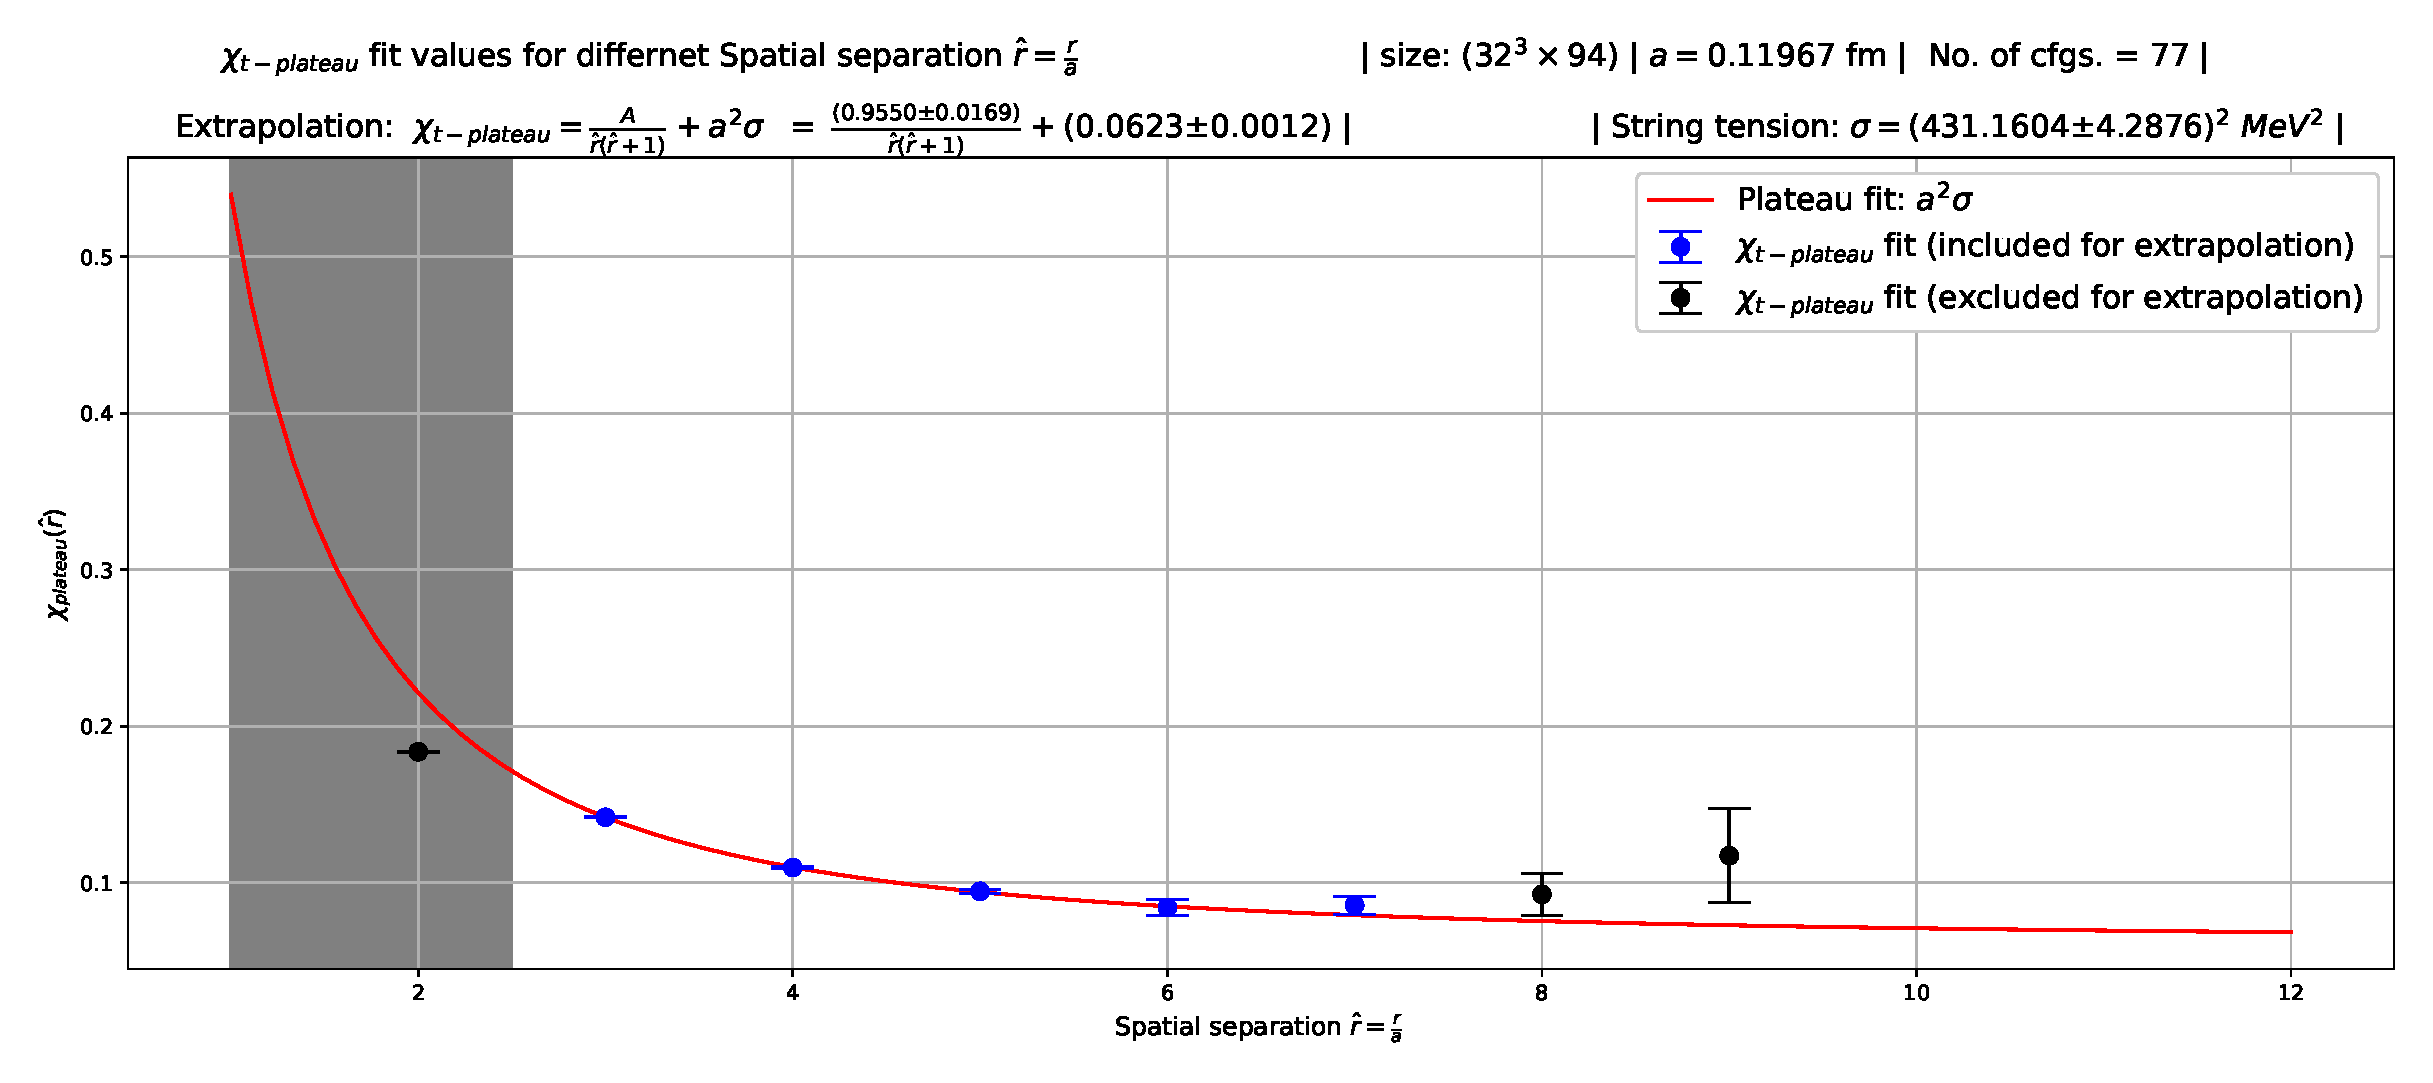
\includegraphics[scale=0.3]{creutzratio.eps}
        \label{fig:enter-label}
    \end{figure}
\end{frame}



\begin{frame}{Proton Two Point Function}
    The proton mass can be determined from the two-point correlation function:
    \begin{align}
        C_{\alpha\beta}(t,\mathbf{p})=a^{3}\sum_{\mathbf{x}}e^{-i\mathbf{p}.\mathbf{x}}C_{\alpha\beta}(t,\mathbf{x})=a^{3}\sum_{\mathbf{x}}e^{-i\mathbf{p}.\mathbf{x}}\bra{0}\chi_{\alpha}(\mathbf{x},t)\widetilde{\chi}_{\beta}(\mathbf{0},0)\ket{0}
    \end{align}
    where
    \begin{align}
        \chi_{\alpha}(\mathbf{x},t)=\epsilon^{ijk}u_{\alpha}^{i}(\mathbf{x},t)u^{j}_{\gamma}(\mathbf{x},t)[C^{-1}\gamma_{5}]_{\gamma\delta}d^{k}_{\delta}(\mathbf{x},t)
    \end{align}
    After integrating out the quark fields in the path integral formulation, this correlator is expressed in terms of products of the inverse of the Dirac operator
    \begin{align*}
        C_{\alpha\beta}(t,\mathbf{p})=&-a^3\sum_{\mathbf{x}}e^{-i\mathbf{p}.\mathbf{x}}\epsilon^{ijk}\epsilon^{i'j'k'}[C^{-1}\gamma_{5}]_{\alpha'\alpha''}[\gamma_{5}C]_{\beta'\beta''}\nonumber\\
        &~~~~~\times\left\langle[\mathcal{M}^{-1}_{d}]^{ki'}_{\alpha''\beta'}\left\{[\mathcal{M}^{-1}_{u}]^{jj'}_{\alpha'\beta''}[\mathcal{M}^{-1}_{u}]^{ik'}_{\alpha\beta}-[\mathcal{M}^{-1}_{u}]^{ij'}_{\alpha\beta''}[\mathcal{M}^{-1}_{d}]^{ik'}_{\alpha'\beta}\right\}\right\rangle
    \end{align*}
    \begin{figure}
    \centering
    \begin{tikzpicture}
        \node (image) {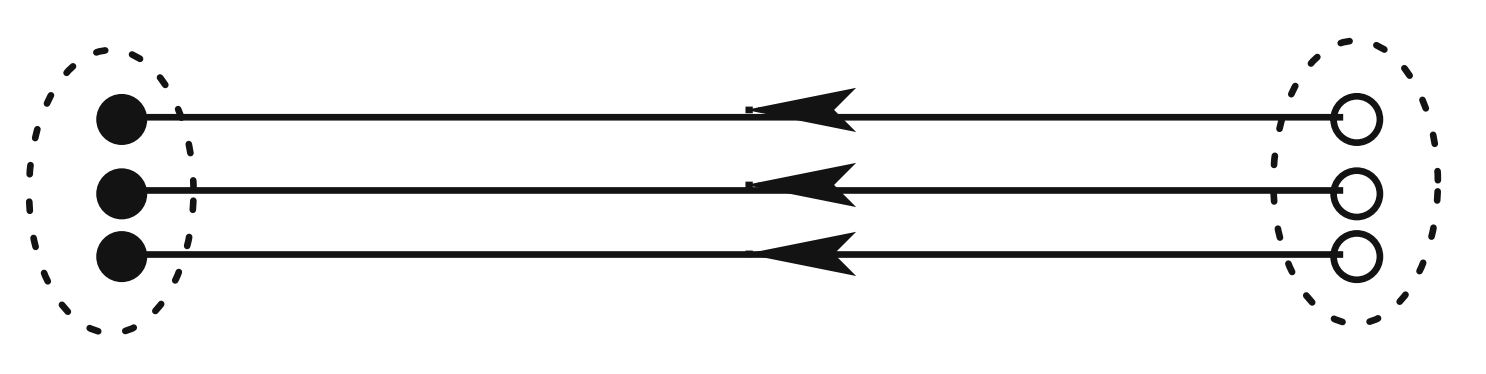
\includegraphics[scale=0.37]{Screenshot 2023-11-07 at 2.50.13 PM.png}};
        % Add annotations using TikZ commands
        \node at (4.3, 0.5) {$u$};
        \node at (4.3, 0) {$u$};
        \node at (4.3, -0.5) {$d$};
        \node at (-4.4, 0.5) {$u$};
        \node at (-4.4, 0) {$u$};
        \node at (-4.4, -0.5) {$d$};
        \node at (-4.1, -1.2) {$(\mathbf{x},t)$};
        \node at (4, -1.2) {$(\mathbf{0},0)$};
        \node at (-0.4, -0.7) {$\mathcal{M}^{-1}_{d}$};
        \node at (-0.4, 0.7) {$\mathcal{M}^{-1}_{u}$};
        \node at (-0.4, 0.2) {$\mathcal{M}^{-1}_{u}$};
    \end{tikzpicture}
    \end{figure}
    
\end{frame}

\begin{frame}{Proton Two Point Function}
    On inserting a complete set of states between the interpolating operators\footnote{Refer: Boussarie, Renaud, et al. "TMD Handbook."	arXiv:2304.03302 [hep-ph].}
    \begin{align}
        C_{\alpha\beta}(t,\mathbf{p})=&a^{3}\sum_{\mathbf{x}}e^{-i\mathbf{p}.\mathbf{x}}\bra{0}\chi_{\alpha}(\mathbf{x},t)\widetilde{\chi}_{\beta}(\mathbf{0},0)\ket{0}\\
        =&a^{3}\sum_{n,\sigma}\frac{e^{-E_{n}(\mathbf{p})t}}{2E_{n}(\mathbf{p})}\bra{0}\chi_{\alpha}\ket{n;\mathbf{p},\sigma}\bra{n;\mathbf{p},\sigma}\widetilde{\chi}_{\beta}\ket{0}\\
        =&a^{3}Z(\mathbf{p})\sum_{\sigma}u_{\alpha}(n=0,\mathbf{p},\sigma)\widetilde{u}_{\beta}(n=0,\mathbf{p},\sigma)\frac{e^{-E_{n}(\mathbf{p})t}}{2E_{n}(\mathbf{p})}+\cdots
    \end{align}
    Tracing this correlator against a given Dirac structure, often chosen to be $\Gamma^{+}=\frac{1}{2}(1+\gamma_{4})$, leads to
    \begin{align}
        \boxed{C_{\Gamma^{+}}(t,\mathbf{p})}=\Gamma^{+}_{\beta\alpha}C_{\alpha\beta}(t,\mathbf{p})\xrightarrow{t\rightarrow\infty}\boxed{Ce^{-E_{n}(\mathbf{p})t}}
    \end{align}
    where $C$ is a time-independent constant.
\end{frame}


\begin{frame}{Proton Two Point Function}
    For $\mathbf{p}=0$ we find $C_{\Gamma^{+}}(t,\mathbf{0})\xrightarrow{t\rightarrow\infty}Ce^{-m_{H}t}$
    \begin{figure}
        \centering
        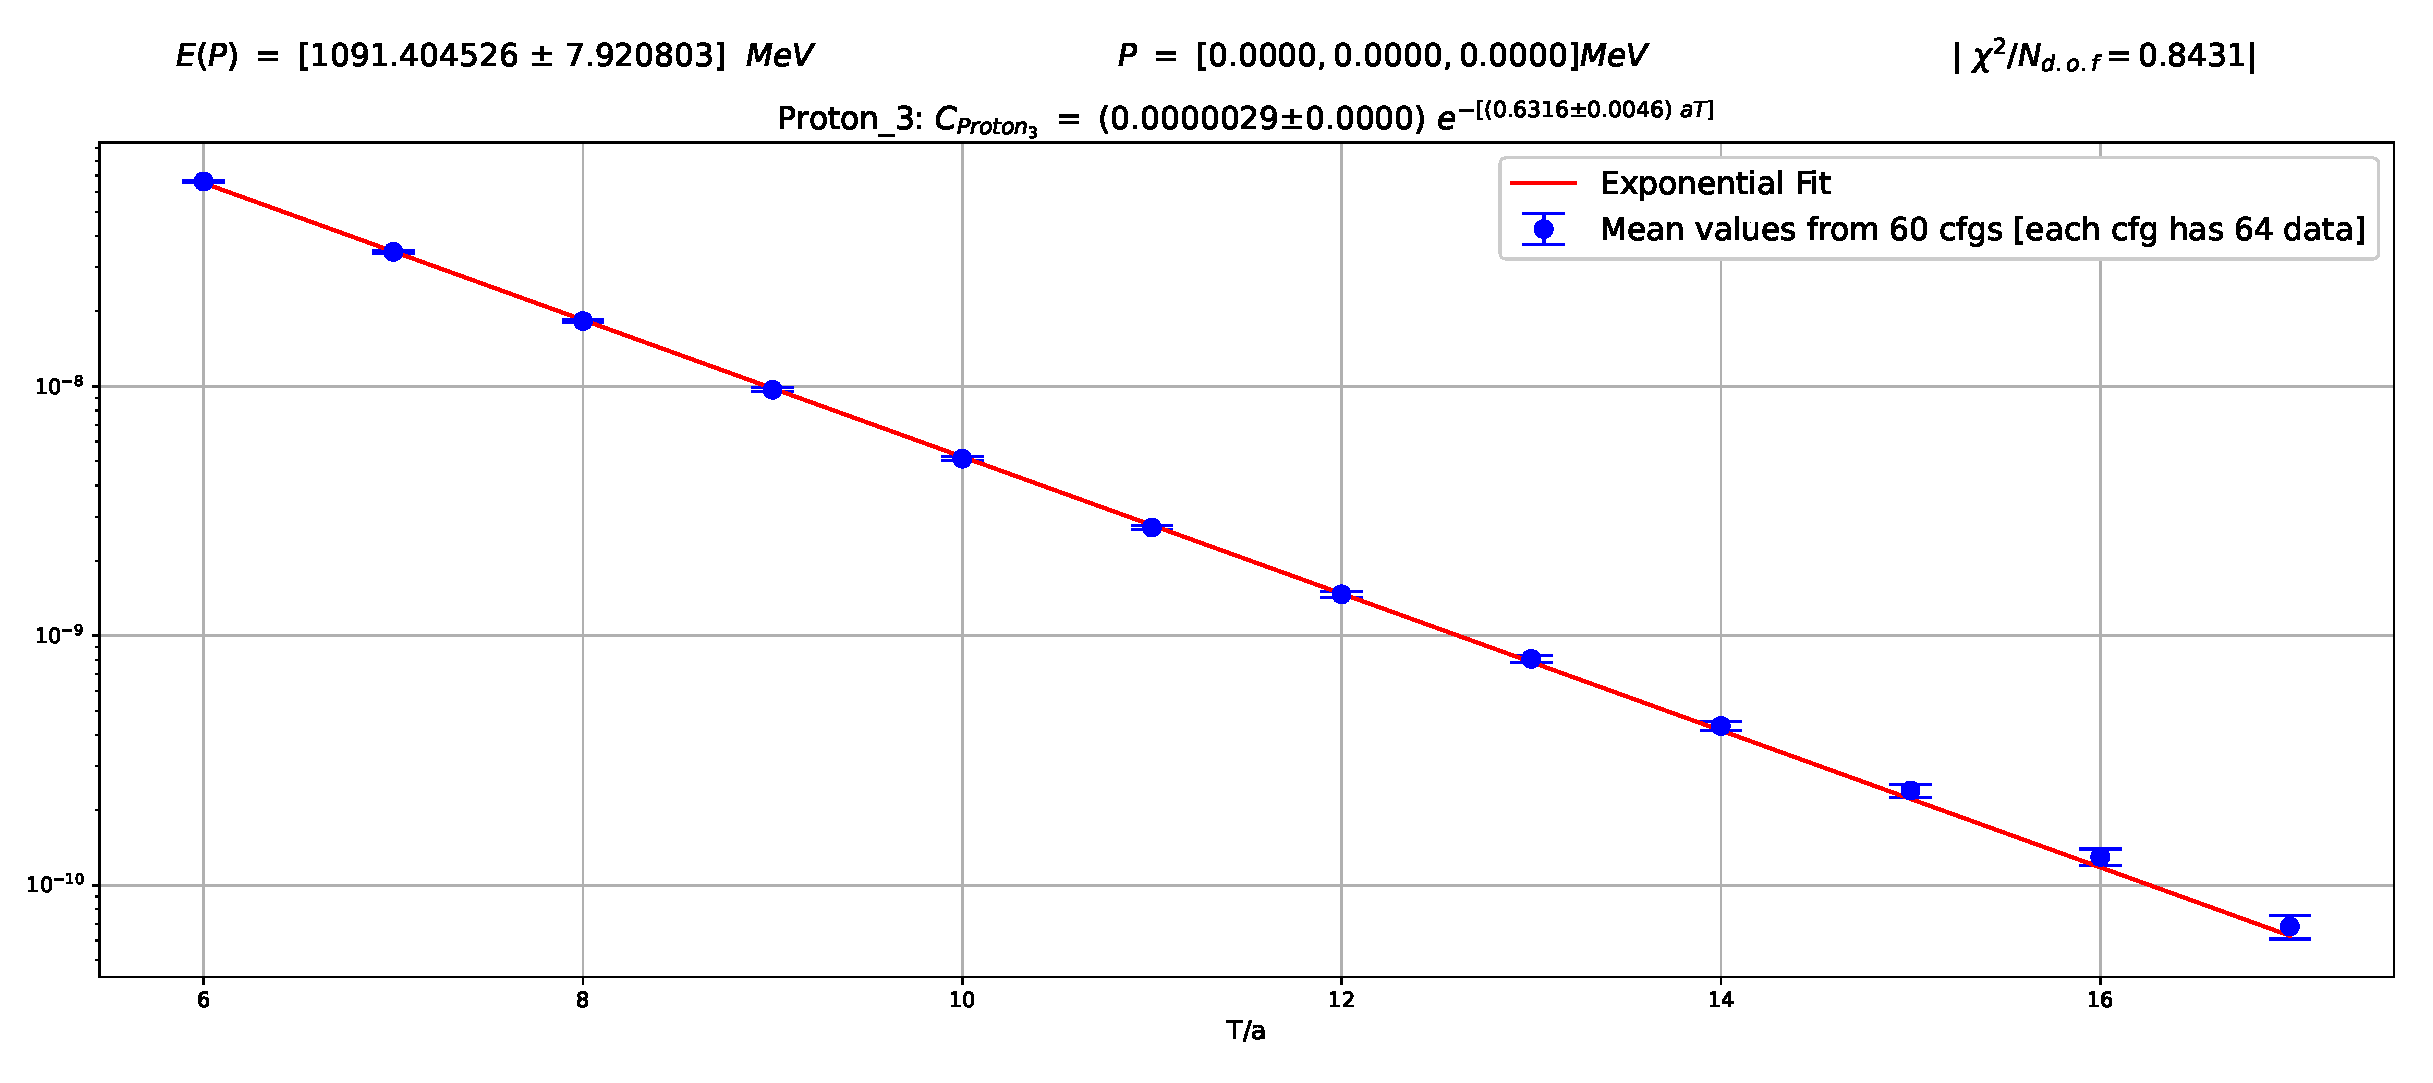
\includegraphics[scale=0.37]{proton3.eps}
        \caption{Proton two-point function $C_{\Gamma^{+}}(t,\mathbf{0})$ from lattice size:$(32^3,94)$ with $a=0.11967~$fm}
        \label{fig:enter-label}
    \end{figure}
\end{frame}


\begin{frame}{Proton Two Point Function}
    Given the discrete time series $C_{\Gamma^{+}}(t,\mathbf{p})$ from the Monte Carlo sampling, the proton mass dispersion relation can be extracted from fits to the time dependence of $C_{\Gamma^{+}}(t,\mathbf{p})\xrightarrow{t\rightarrow\infty}Ce^{-E_{n}(\mathbf{p})t}$:
    \begin{figure}
        \centering
        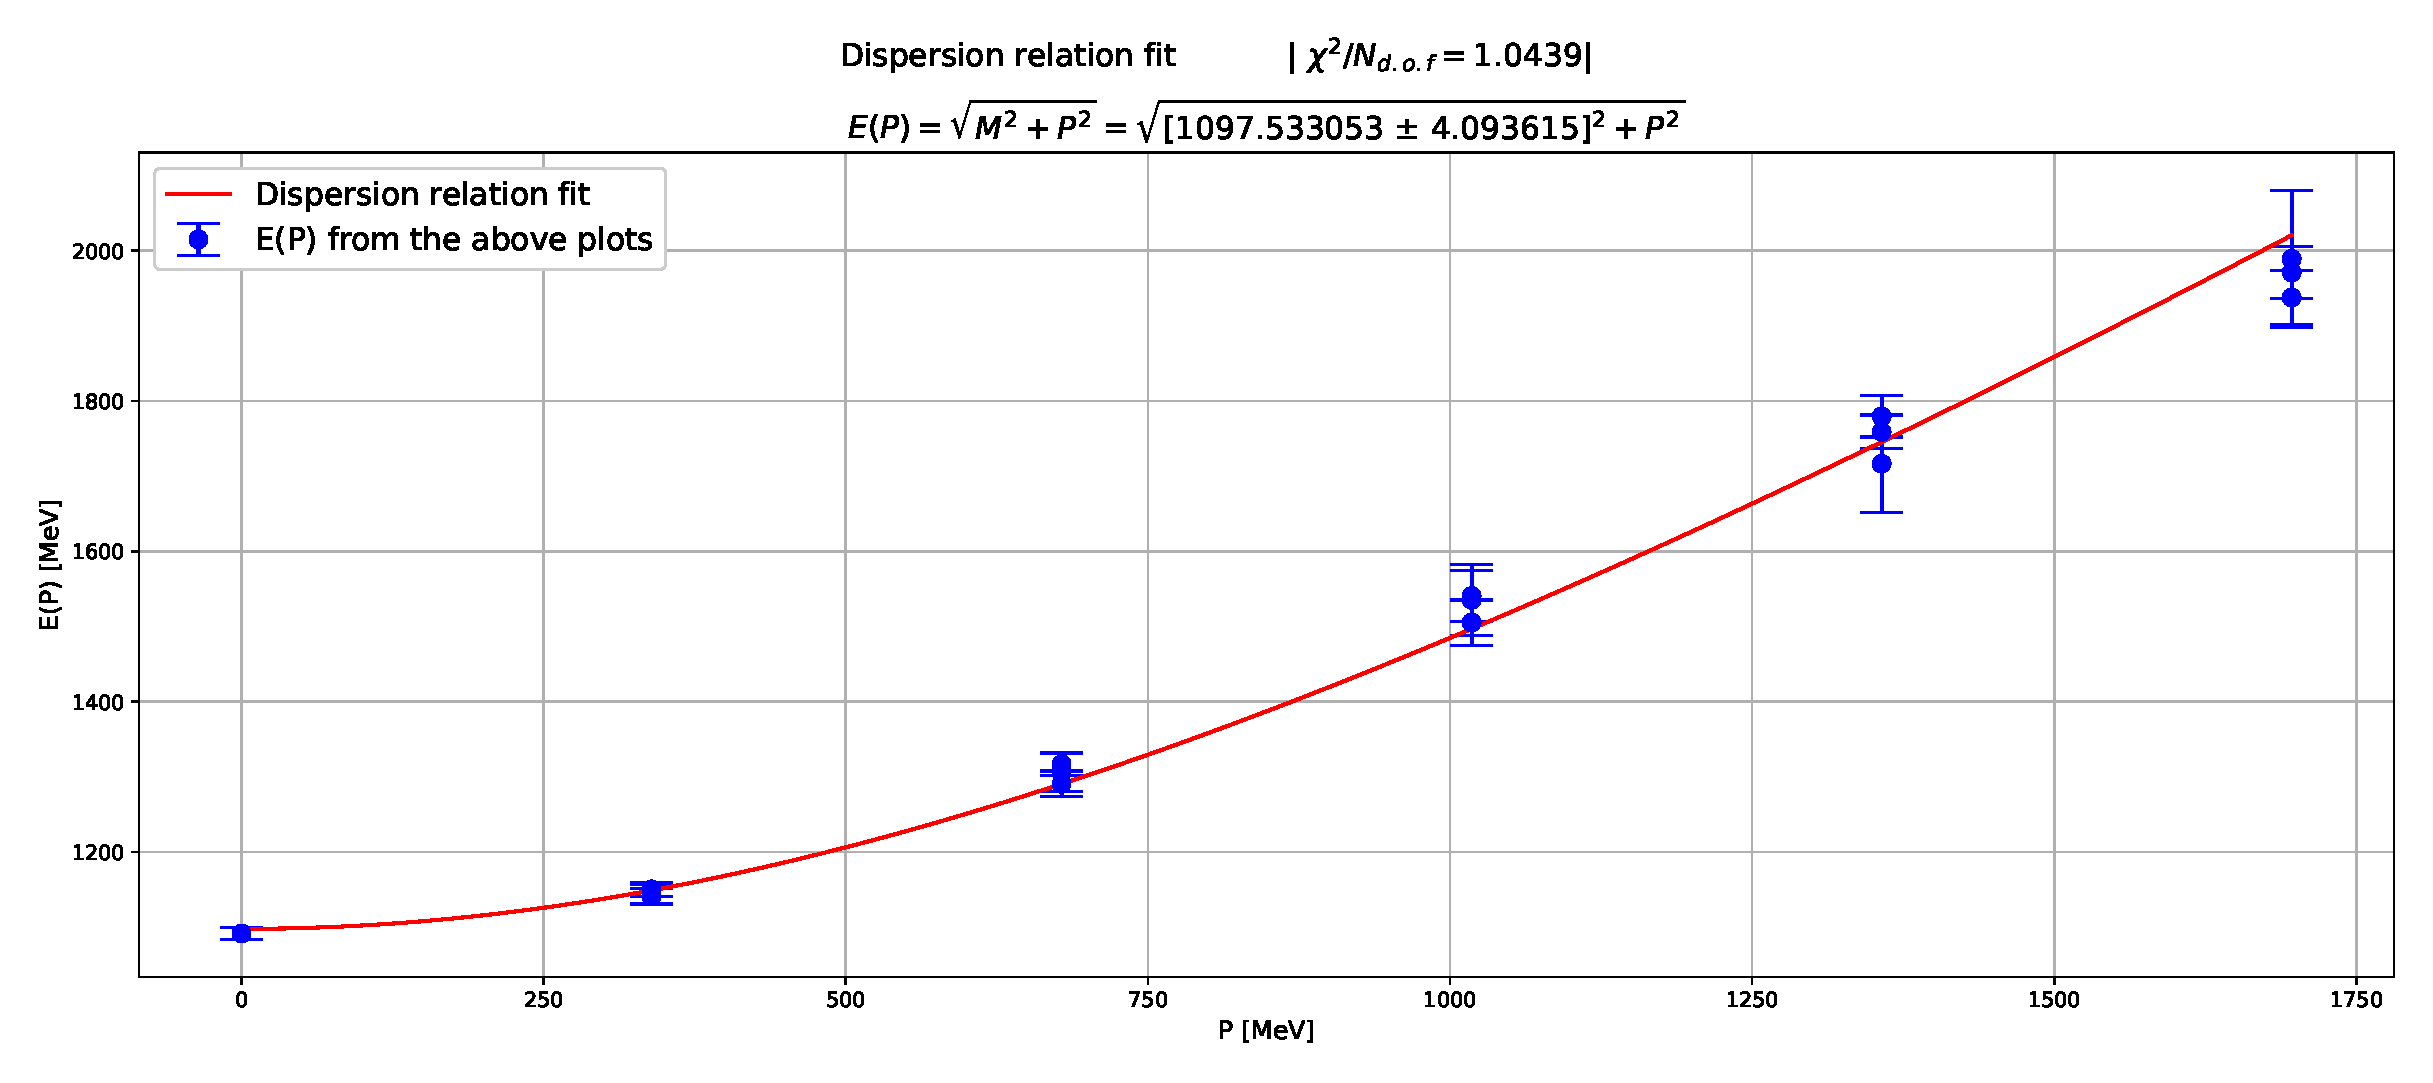
\includegraphics[scale=0.36]{dispersion_.eps}
        \caption{Proton dispersion relation from lattice size:$(32^3,94)$ with $a=0.11967~$fm}
        \label{fig:enter-label}
    \end{figure}
\end{frame}



\begin{frame}{Introduction: TMDs}
The \textbf{intrinsic motion of quarks and gluons} inside the proton or neutron, specifically \textbf{with respect to the transverse momentum}, can be described in terms of Transverse Momentum Dependent Parton Distribution Functions (TMDs)

\begin{figure}[!]
     \centering
     \begin{subfigure}[b]{0.35\textwidth}
         \centering
         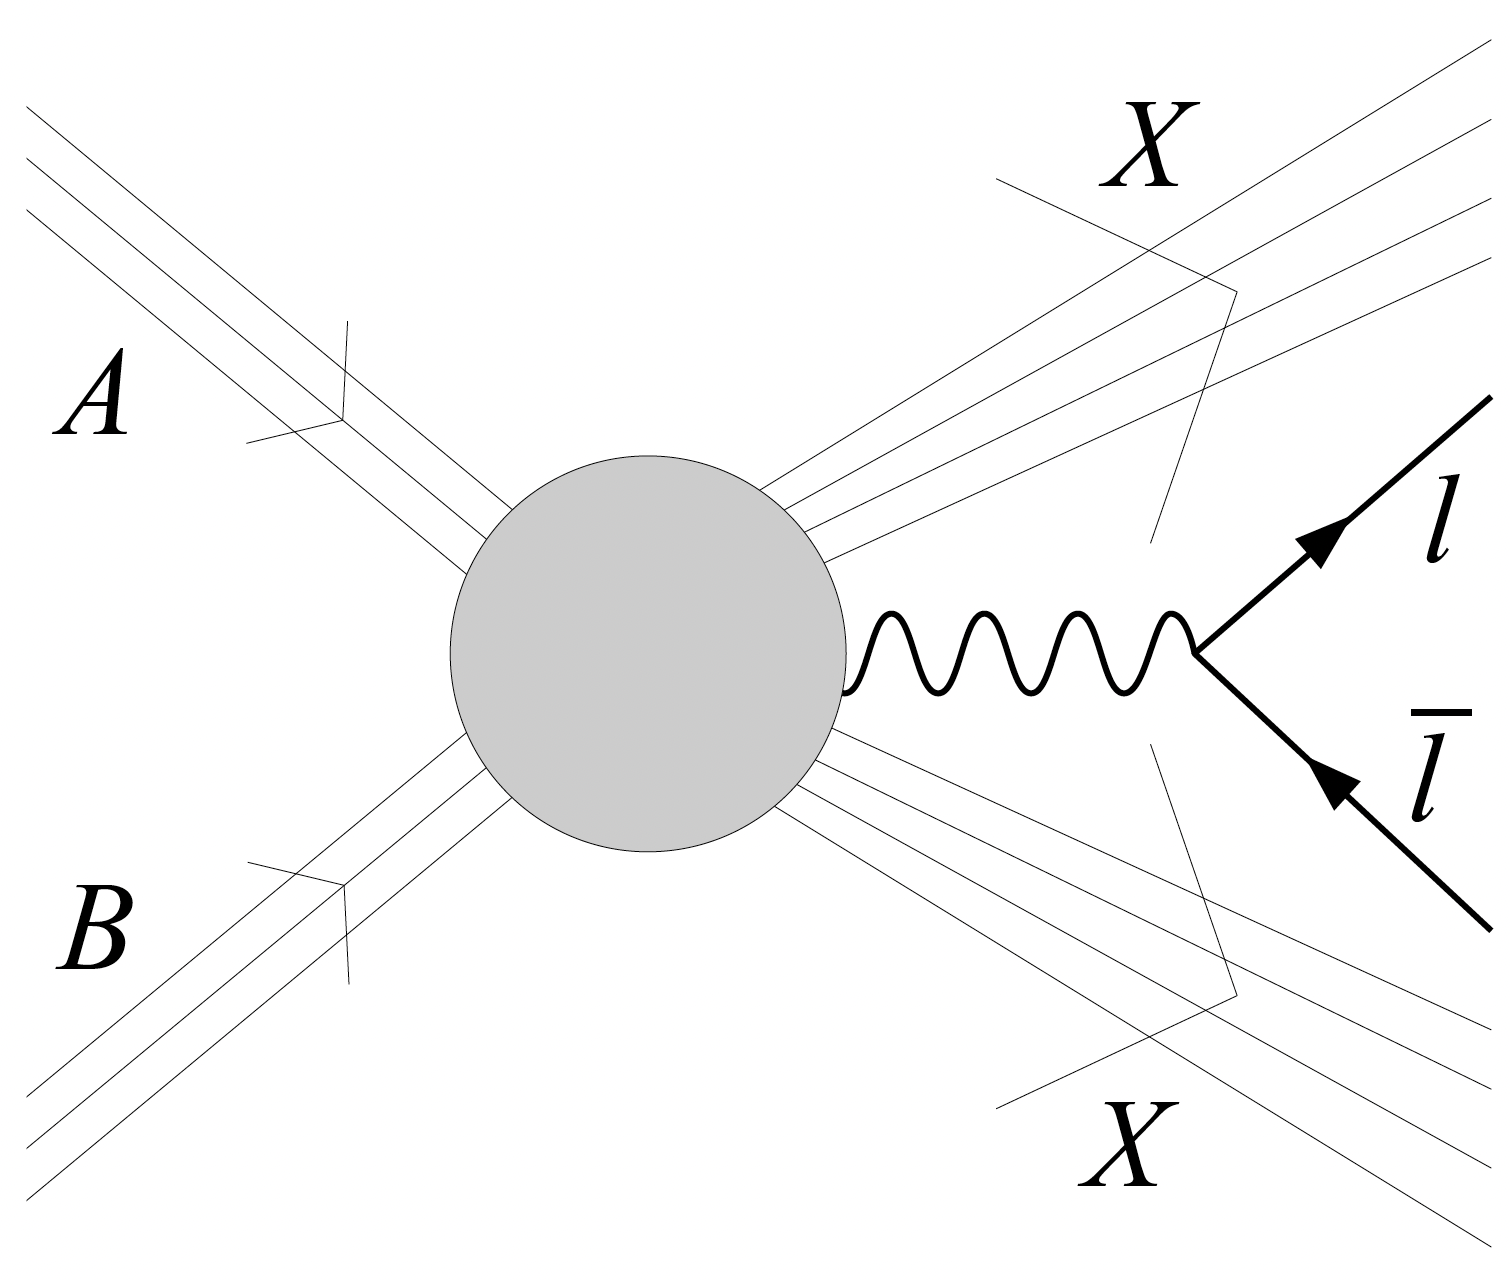
\includegraphics[width=\textwidth]{Screenshot 2023-06-13 at 10.31.01 PM.png}
         \caption{The Drell-Yan process.}
         \label{fig:y equals x}
     \end{subfigure}
     \begin{subfigure}[b]{0.35\textwidth}
         \centering
         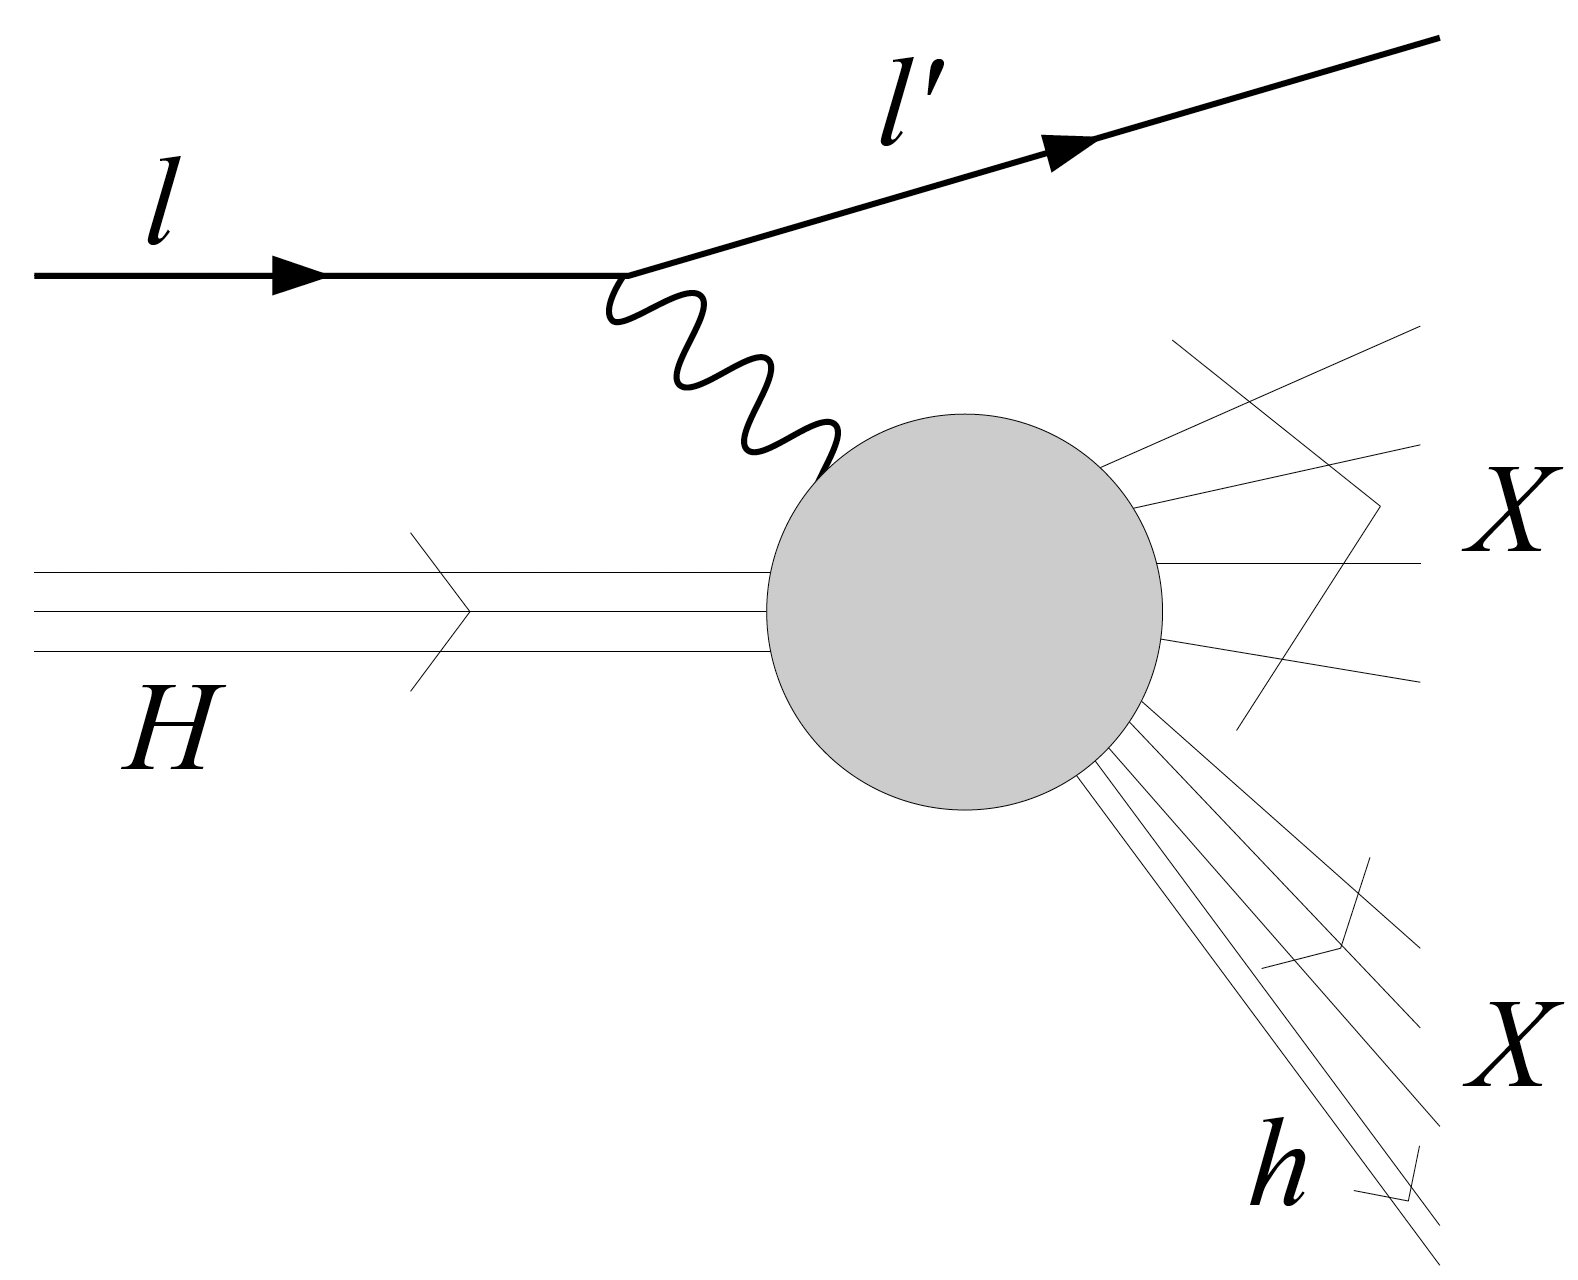
\includegraphics[width=\textwidth]{Screenshot 2023-06-13 at 10.31.19 PM.png}
         \caption{The SIDIS process.}
         \label{fig:three sin x}
     \end{subfigure}
        \caption{Two examples of processes sensitive to TMD PDFs. We draw the leading contributions, in which a single electroweak gauge boson (wiggled lines) is exchanged.}
        \label{fig:three graphs}
\end{figure}


\end{frame}



\begin{frame}{Introduction: TMDs}
In the SIDIS cross section
\begin{align}
    \frac{d\sigma}{d^3P_h d^3P_{l'}}\propto L_{\mu\nu}W^{\mu\nu}
\end{align}
\begin{align}
    \Longrightarrow~~W^{\mu\nu}(P,q,P_h)=&\int \frac{d^4l}{(2\pi)^4}e^{iq\cdot l}\sum_{X}\bra{N(P,S)}J^{\mu}(-b)\ket{Xh(P_h,S_h)}\bra{Xh(P_h,S_h)}J^{\nu}(0)\ket{N(P,S)}\nonumber
\end{align}
\begin{figure}
    \centering
    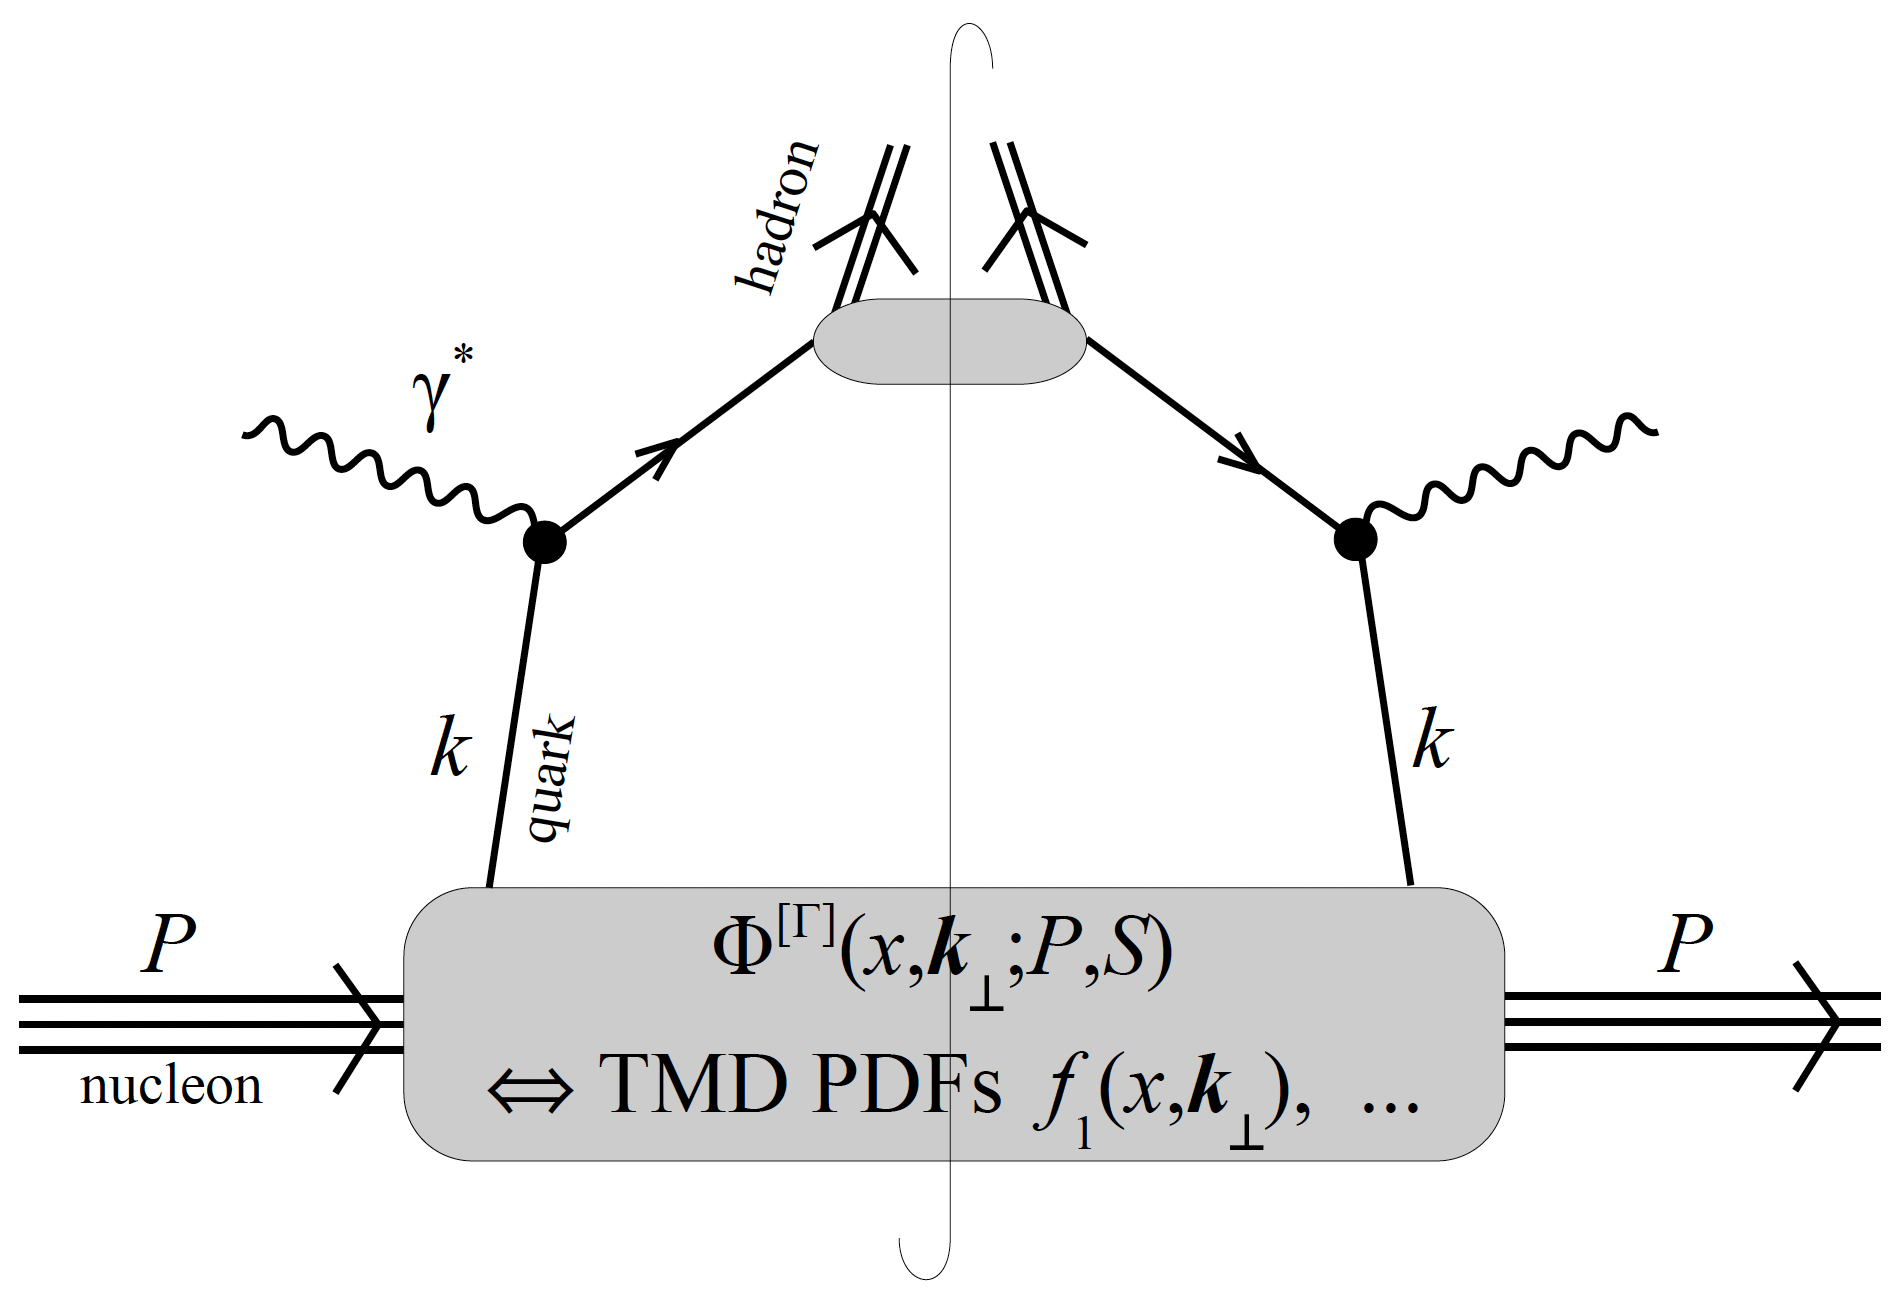
\includegraphics[scale=0.2]{Screenshot 2023-06-13 at 10.24.44 PM.png}
    \caption{Simplifed factorized tree level diagram of the hadron tensor in SIDIS. ~~\textit{arXiv:0907.2381}}
\end{figure}
\end{frame}


\begin{frame}{Definition of TMDs}

\begin{itemize}
    \item Consider a frame where the nucleon has large momentum in $z$-direction, i.e., $P^+ \gg m_N$, $\vprp{P} = 0$.
In light cone coordinates, the components \textcolor{brown}{\boxed{$\kei^+$:~$\vprp{\kei}$:~$\kei^-$ $\sim$ $P^+/m_N$:~$1$:~$m_N/P^+$}}, under boosts along the $z$-axis.
\end{itemize}
The starting point for our discussion of TMDs are the correlator of the general form

\begin{align}
	\Phi^{[\Gamma]}(\kei,P,S;\ldots)\ \equiv\ \ 
	\int \frac{d^4 \bvec}{(2\pi)^4}\, e^{i \kei\cdot \bvec}\,
		\frac{\overbrace{\rule{0em}{1.2em}
		\frac{1}{2}\, \bra{P,S}\ \bar{q}(0)\, \Gamma\ \textcolor{blue}{\WlineC{\mathcal{C}_\bvec}}\ q(\bvec)\ \ket{P,S}
		}^{\displaystyle \equiv \widetilde \Phi_\unsub^{[\Gamma]}(\bvec,P,S;\ldots)}}
		{ \widetilde{\softf}(\bvec^2;\ldots) }
		%{ \underbrace{ \widetilde{\mathcal{S}}(\elll^2,\ldots) }_{\displaystyle \text{soft factor}}}
		\label{eq-corr}	
\end{align}

\begin{itemize}
    \item The gauge link \textcolor{blue}{$\WlineC{\mathcal{C}_\bvec}$} brings divergences; so we divide it by soft factor $\tilde \softf$
\end{itemize}
\end{frame}



\begin{frame}{Definition of TMDs}
Integrating the correlator over the suppressed momentum component $k^-$ yields 
\begin{align}
	\resizebox{0.2\hsize}{!}{\Phi^{[\Gamma]}(x,\vprp{k};P,S;\ldots) }& \equiv \resizebox{0.2\hsize}{!}{\int dk^{-} \Phi^{[\Gamma]}(\kei,P,S;\ldots)} \nonumber \\ 
	& =\resizebox{0.7\hsize}{!}{\int \frac{d^2 \vprp{\bvec}}{(2\pi)^2} \int \frac{d (\bvec \tcdot P)}{(2\pi) P^+}\ e^{i x (\bvec \tcdot P) - i\vprp{\bvec} \tcdot \vprp{\kei}}\,
		\left. \frac{\frac{1}{2}\, \bra{P,S}\ \bar{q}(0)\, \Gamma\ \textcolor{blue}{\WlineC{\mathcal{C}_\bvec}}\ q(\bvec)\ \ket{P,S}}
		{ \widetilde{\mathcal{S}}(-\vprp{\bvec}^2;\ldots) } \right|_{b^+ = 0} \ }.
\end{align}
The above correlator can be decomposed into \TMDs.
\begin{align}
	\Phi^{[\gamma^+]}(x,\vprp{k};P,S,\ldots) & = \textcolor{red}{f_1} - \toddmark{\frac{\myeps_{ij}\, \vect{k}_{i}\, \vect{S}_{j}}{m_N}\ \textcolor{red}{f_{1T}^\prp}} \label{eq-phigammaplus}\ , \displaybreak[0]  \\ 
	\Phi^{[\gamma^+\gamma^5]}(x,\vprp{k};P,S,\ldots) & = \Lambda\,\textcolor{red}{ g_{1}} + \frac{\vprp{k} \cdot \vprp{S}}{m_N}\ \textcolor{red}{g_{1T}} \label{eq-phigammaplusgfive} \ , \displaybreak[0] \\
	\Phi^{[i\sigma^{i+}\gamma^5]}(x,\vprp{k};P,S,\ldots) & = \vect{S}_i\ \textcolor{red}{h_{1}}   +  \frac{(2 \vect{k}_i \vect{k}_j - \vprp{k}^2 \delta_{ij}) \vect{S}_j}{2 m_N^2}\, \textcolor{red}{h_{1T}^\prp} \nonumber \\
 &~~~~~~~~~+ \frac{\Lambda \vect{k}_i}{m_N} h_{1L}^\prp +   \toddmark{\frac{\myeps_{ij} \vect{k}_{j}}{m_N} \textcolor{red}{h_1^\prp}}\ .\label{eq-phisigmaplusi} 
\end{align}

\end{frame}


\begin{frame}{Parametrization of the correlator in position space}
\begin{align}
    {\widetilde \Phi_\unsub^{[\Gamma]}(\bvec,P,S,\hat \zeta, \mu)}
		\equiv\frac{1}{2}\, \bra{P,S}\ \bar{q}(0)\, \Gamma\ \textcolor{blue}{\Wline{0, \eta v, \eta v + b, b}}\ q(\bvec)\ \ket{P,S}
\end{align}

For the $\Gamma$-structures at leading twist, the correlator can be written in the form 
\begin{align}
	\frac{1}{2 P^+}\widetilde \Phi^{[\gamma^+]}_{\unsub} & = 	
		\textcolor{red}{\tAmp_{2B} }
		+ i \mN \epsilon_{ij} \vect{\bvec}_i \vect{S}_j\, \textcolor{red}{\tAmp_{12B} }
		\displaybreak[0] \\
	\frac{1}{2 P^+}\widetilde \Phi^{[\gamma^+ \gamma^5]}_{\unsub} & = 
		- \Lambda\, \textcolor{red}{\tAmp_{6B} }
		+ i \left\{ (\bvec \tcdot P) \Lambda - \mN (\vprp{\bvec} \tcdot \vprp{S}) \right\}\, \textcolor{red}{\tAmp_{7B}}
		\displaybreak[0] \\
	\frac{1}{2 P^+}\widetilde \Phi^{[i \sigma^{i+} \gamma^5]}_{\unsub} & = 
		i \mN \epsilon_{ij} \vect{\bvec}_j \, \textcolor{red}{\tAmp_{4B} }
		- \vect{S}_i\, \textcolor{red}{\tAmp_{9B} }
		- i\mN \Lambda \vect{\bvec}_i\, \textcolor{red}{\tAmp_{10B}}
		\nonumber\\
  &~~~~~~+ \mN \left\{ (\bvec \tcdot P) \Lambda - \mN (\vprp{\bvec} \tcdot \vprp{S}) \right\} \vect{b}_i\, \textcolor{red}{\tAmp_{11B}}
\end{align}

(Decompositions analogous to work by Metz et al. Phys. Lett. \textbf{B618} (2005) 90-96. in momentum space)
\end{frame}



\begin{frame}{Strategy}
  \begin{figure}
    \centering
    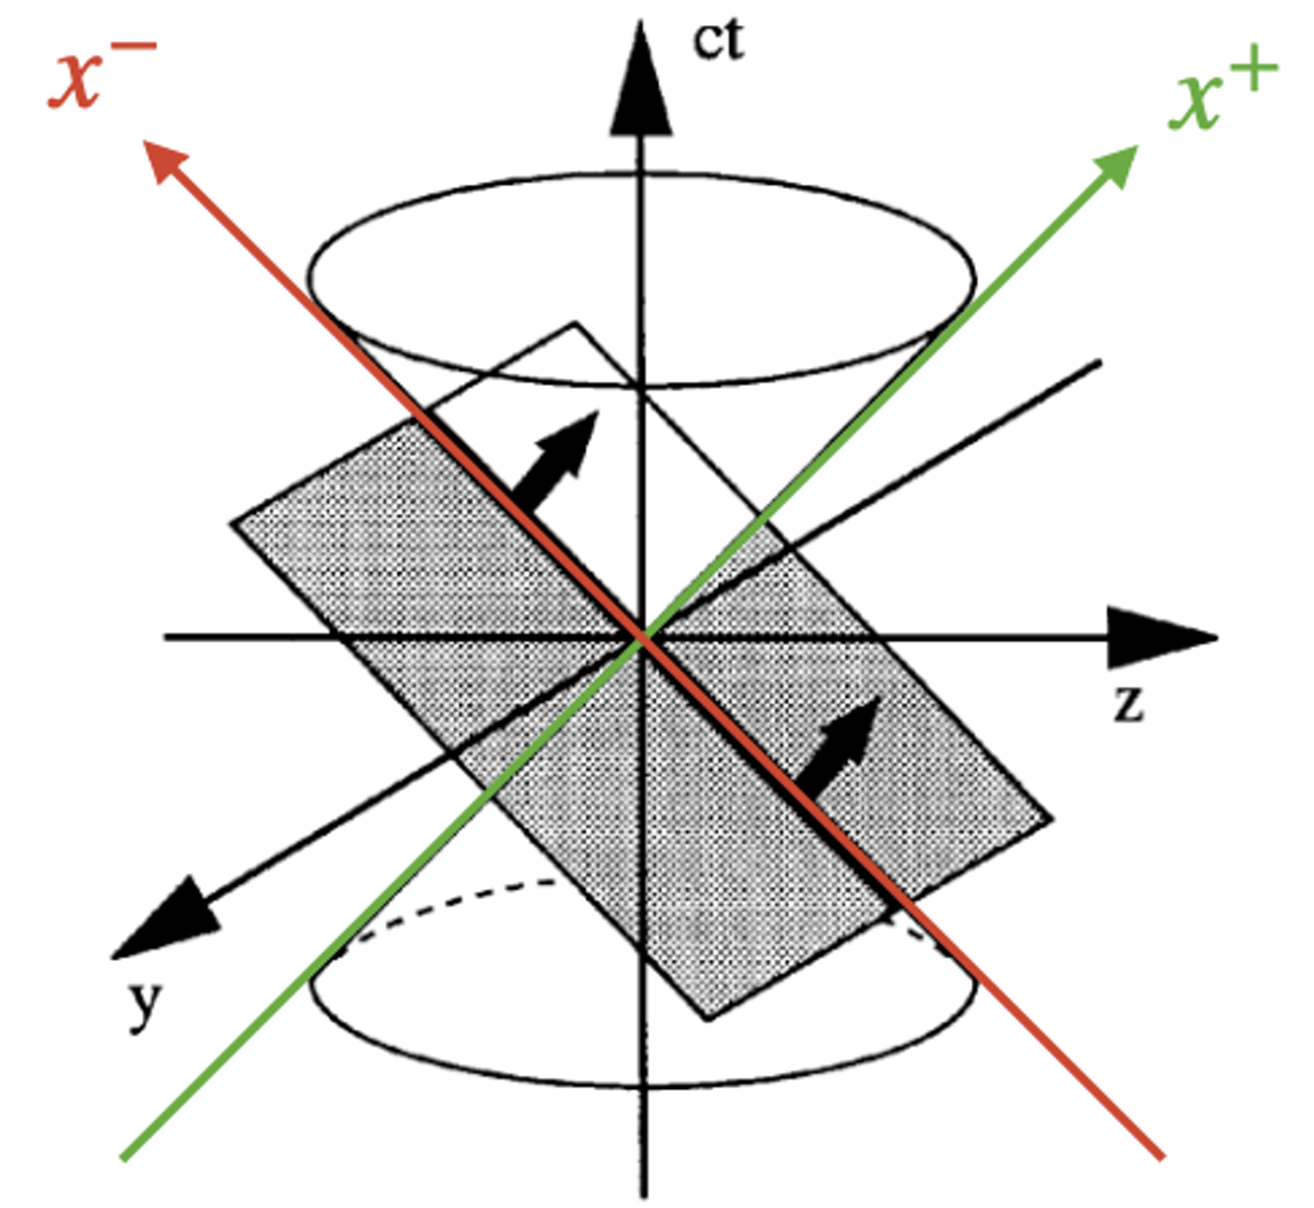
\includegraphics[scale=0.1]{Screenshot 2023-06-14 at 3.10.53 PM.png}
    \caption{Light-front coordinates}
    \label{fig:enter-label}
\end{figure}
    \begin{itemize}
        \item The separation $b$ of the quark field operators has a transverse component, $\boxed{\bvec = n \bvec^- + \bvec_\perp}$. So, this separation is space-like
        \begin{align}
	\Phi^{[\Gamma]}(\kei,P,S;\ldots)\ \equiv\ \ 
	\int \frac{d^4 \bvec}{(2\pi)^4}\, e^{i \kei\cdot \bvec}\,
		\frac{\overbrace{\rule{0em}{1.2em}
		\frac{1}{2}\, \bra{P,S}\ \bar{q}(0)\, \Gamma\ \textcolor{blue}{\WlineC{\mathcal{C}_\bvec}}\ q(\bvec)\ \ket{P,S}
		}^{\displaystyle \equiv \widetilde \Phi_\unsub^{[\Gamma]}(\bvec,P,S;\ldots)}}
		{ \widetilde{\softf}(\bvec^2;\ldots) }
		%{ \underbrace{ \widetilde{\mathcal{S}}(\elll^2,\ldots) }_{\displaystyle \text{soft factor}}}
		\label{eq-corr}	
        \end{align}
        \item We \textcolor{red}{parametrized} this correlator \textcolor{red}{in terms of Lorentz-invariant amplitudes}
        \item We choose the Lorentz frame in which this nonlocal operator is defined \textcolor{red}{at one single time}
        \item The computation of the nonlocal matrix element can be cast in terms of a \textcolor{red}{Euclidean path integral and performed employing the standard methods of lattice QCD}
    \end{itemize}
\end{frame}

\begin{frame}{Link geometry}
The gauge link employed in this work reads
\begin{align}
	\textcolor{blue}{\WlineC{\mathcal{C}_\bvec^{(\eta v)}}} = \textcolor{blue}{\Wline{0, \eta v, \eta v + b, b}} ,
	\label{eq-staplelink}
\end{align}

\begin{figure}
    \centering
    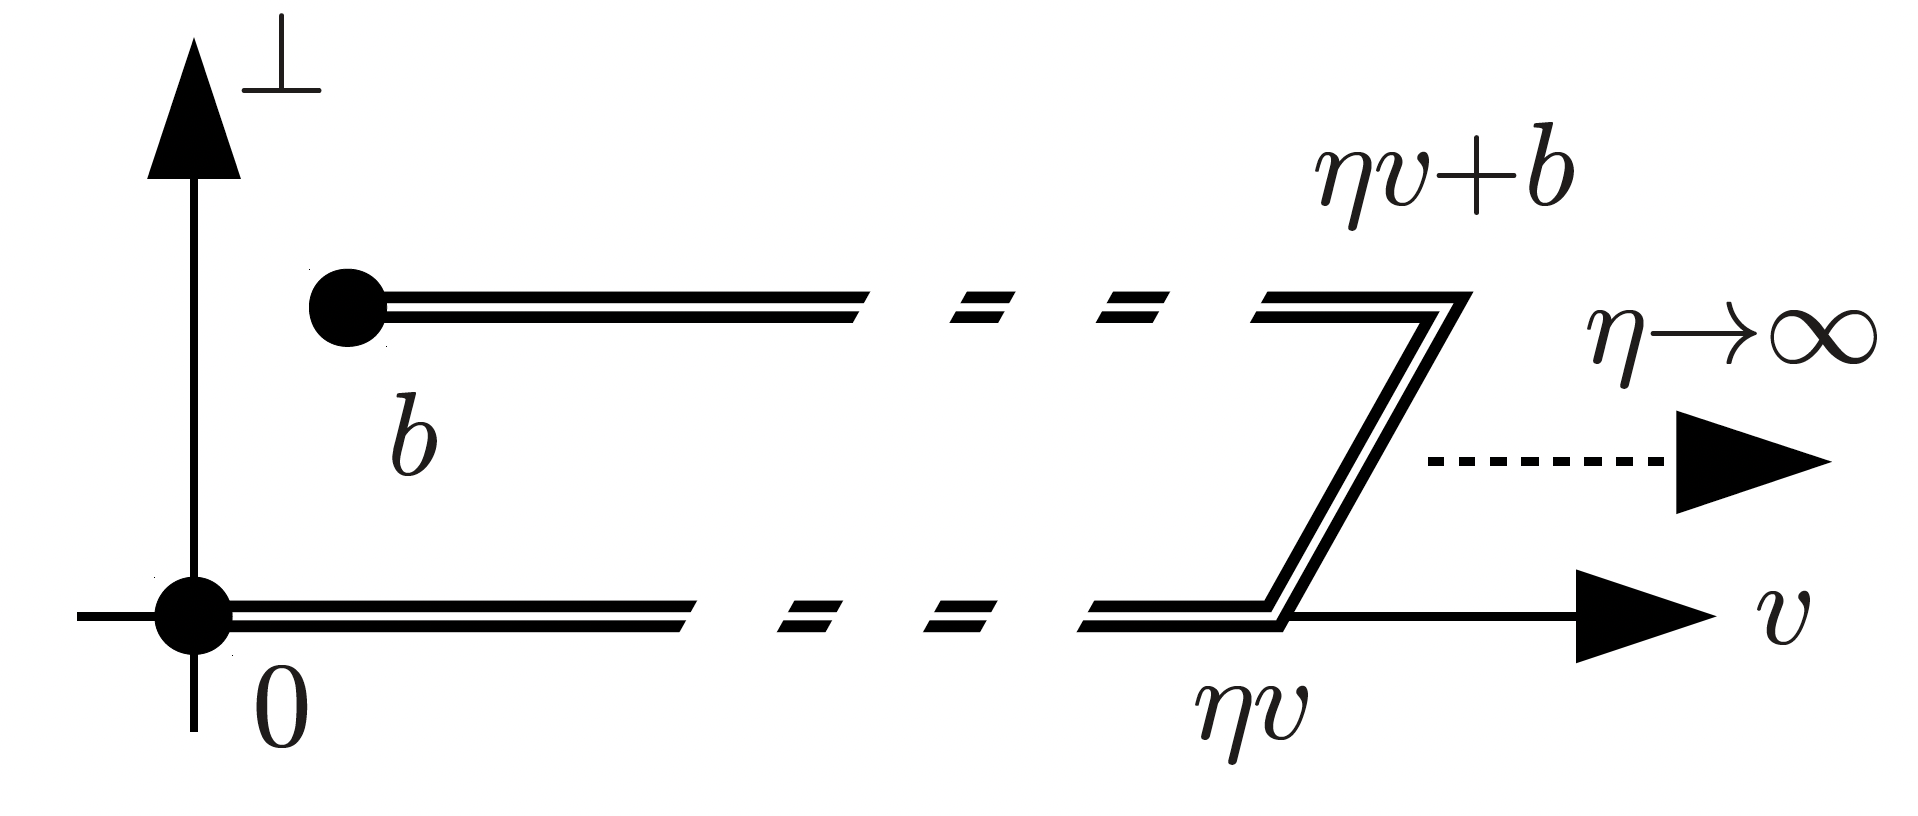
\includegraphics[scale=0.12]{Screenshot 2023-06-14 at 10.33.12 AM.png}
    \caption{Staple-shaped
gauge connection. The four-vectors $v$ and $P$ give the direction of the staple and the momentum, while b defines the separation between the quark operators. \textit{(arXiv:1111.4249v2 [hep-lat])}}
    \label{fig:enter-label}
\end{figure}


The Lorentz-invariant quantity characterizing the direction of $v$ is the Collins-Soper type parameter
\begin{equation}
	\boxed{\hat \zeta \equiv \zeta / 2 \mN =  \frac{v \cdot P}{\sqrt{|v^2|} \sqrt{P^2}}.}
	\label{eq-zeta}
\end{equation}

The light-like direction $v = \nminus$ can be approached in the limit $\zeta \rightarrow \infty$.
\end{frame}



\begin{frame}{TMDs in Fourier space and $x$-integrations (Mellin moments)}
\begin{align}
    \tilde f(x, \vprp{\bvec}^2;\ldots) & \equiv \int  d^2 \vprp{\kei} \, e^{i \vprp{\bvec} \cdot \vprp{\kei} }\; f(x, \vprp{\kei}^2;\ldots)\\
    \tilde f^{(n)}(x, \vprp{\bvec}^2\ldots ) & \equiv n!\left( -\frac{2}{\mN^2}\partial_{\vprp{\bvec}^2} \right)^n \ 
	\tilde f(x, \vprp{\bvec}^2;\ldots ) 
\end{align}
 In the limit $|\vprp{\bvec}| \rightarrow 0$, one recovers conventional $\vprp{\kei}$-moments of \TMDs:
\begin{align}
	\tilde f^{(n)}(x, 0;\ldots ) & = \int  d^2 \vprp{\kei} \left( \frac{\vprp{\kei}^2}{2 \mN^2 }\right)^n  f(x, \vprp{\kei}^2;\ldots ) \equiv  f^{(n)}(x)\ .
	\label{eq-btder2}
\end{align}
$\vprp{\kei}$-moments like $f_1^{(0)}(x)$ and $f_{1T}^{\perp(1)}(x)$ are ill-defined without further regularization, we therefore do not attempt to extrapolate to $\vprp{\bvec}=0$, but rather state our results at finite $|\vprp{\bvec}|$.\\

\textcolor{red}{\textbf{In our studies so far, we only considered the first $x$-moments (accessible at $b \cdot P = 0$), rather than scanning range
of $b \cdot P$}}
\begin{align}
	f^{[1]}(\vprp{\kei}^2;\ldots) \equiv \int_{-1}^1 dx\ f(x,\vprp{\kei}^2;\ldots)\ .
\end{align}
where, $x=\frac{k^{+}}{P^{+}}$
\end{frame}

%\begin{frame}{T-even and T-odd TMDs}
%    The T-even distributions $f_1$, $g_1$, $h_1$, $g_{1T}$, $h_{1L}^\perp$ and $h_{1T}^\perp$ fulfill
%\begin{align}
%	\boxed{ f^{\text{T-even}}(x,\vprp{\kei}^2;\zetahat,\ldots,\eta v \tcdot P) = f^{\text{T-even}}%(x,\vprp{\kei}^2;\zetahat,\ldots,-\eta v \tcdot P)}
%\end{align}
%while the T-odd distributions, i.e., at leading twist the Sivers function $f_{1T}^\perp$ and the Boer-Mulders function %$h_{1}^\perp$, fulfill
%\begin{align}
%	\boxed{ f^{\text{T-odd}}(x,\vprp{\kei}^2;\zetahat,\ldots,\eta v \tcdot P)  = - f^{\text{T-odd}}%(x,\vprp{\kei}^2;\zetahat,\ldots,-\eta v \tcdot P)}
%\end{align}
%As a result, T-odd distributions must vanish for $\eta = 0$, which corresponds to straight gauge links.
%\end{frame}



\begin{frame}{TMDs in Fourier space and invariant amplitudes \textcolor{red}{$\tAmp_i(\bvec^2,\bvec \tcdot P,(\bvec \tcdot P) R(\zetahat^2)/\mN^2,-1/(\mN\zetahat)^2,\eta v \tcdot P)$}}
    Certain $x$-integrated TMDs in Fourier space directly correspond to the amplitudes \textcolor{red}{$\tAmp_{iB}$} evaluated at $\bvec \tcdot P = 0$ :
   \begin{align}
	\tilde f_1^{[1](0)}(\vprp{\bvec}^2;\zetahat,\ldots,\eta v \tcdot P) & = 2\, \textcolor{red}{\widetilde{A}_{2B}(-\vprp{\bvec}^2,0,0,-1/(\mN\zetahat)^2,\eta v\tcdot P)}/\widetilde{\mathcal{S}}(\bvec^2;\ldots) \,,\nonumber  \\
	\tilde f_{1T}^{\perp[1](1)}(\vprp{\bvec}^2;\zetahat,\ldots,\eta v \tcdot P) & =-2 \,\textcolor{red}{\widetilde{A}_{12B}(-\vprp{\bvec}^2,0,0,-1/(\mN\zetahat)^2,\eta v\tcdot P)}/\widetilde{\mathcal{S}}(\bvec^2;\ldots) \,,\nonumber
	\label{eq-xintderfttmds}
   \end{align} 
\end{frame}


\begin{frame}{Generalized Sivers shifts from amplitudes}
All other renormalization and soft factor related dependences cancel out in the ratio.

\begin{itemize}
    \item  $\langle \vect{k}_y \rangle^{\text{Sivers}}=\langle \vect{k}_y \rangle_{TU}$ is T-odd, it describes a feature of the transverse momentum distribution of (unpolarized) quarks in a transversely polarized proton. 
\end{itemize}
\begin{align}
    \langle \vect{k}_y \rangle_{TU}(\vprp{\bvec}^2;\zetahat,\eta v \tcdot P) 
	&\ \equiv\ \mN \frac{\tilde f_{1T}^{\perp[1](1)}(\vprp{\bvec}^2;\zetahat,\ldots,\eta v \tcdot P)}{\tilde f_1^{[1](0)}(\vprp{\bvec}^2;\zetahat,\ldots,\eta v \tcdot P)}  
	\nonumber \\
 &~~= - \mN \frac{\textcolor{red}{\widetilde{A}_{12B}(-\vprp{\bvec}^2,0,0,-1/(\mN\zetahat)^2,\eta v\tcdot P)} }{ \textcolor{red}{\widetilde{A}_{2B}(-\vprp{\bvec}^2,0,0,-1/(\mN\zetahat)^2,\eta v\tcdot P) }} \nonumber \\
	&\ \xrightarrow{\vprp{\bvec}^2 = 0} 
		\left. \frac{ \int dx \int d^2 \vprp{\kei}\, \vect{\kei}_y  \ \Phi^{[\gamma^+]}(x,\vprp{\kei},P,S;\ldots) }
		{ \int dx \int d^2 \vprp{\kei}  \phantom{\vect{\kei}_y}\ \Phi^{[\gamma^+]}(x,\vprp{\kei},P,S;\ldots) } \right|_{\displaystyle \vprp{S}=(1,0) } 
	\label{eq-genSivShift} 
\end{align}
\end{frame}






\begin{frame}{Lattice Setup \footnote{Figure Credits: Dr. Engelhardt (NMSU)}}
\begin{figure}
    \centering
    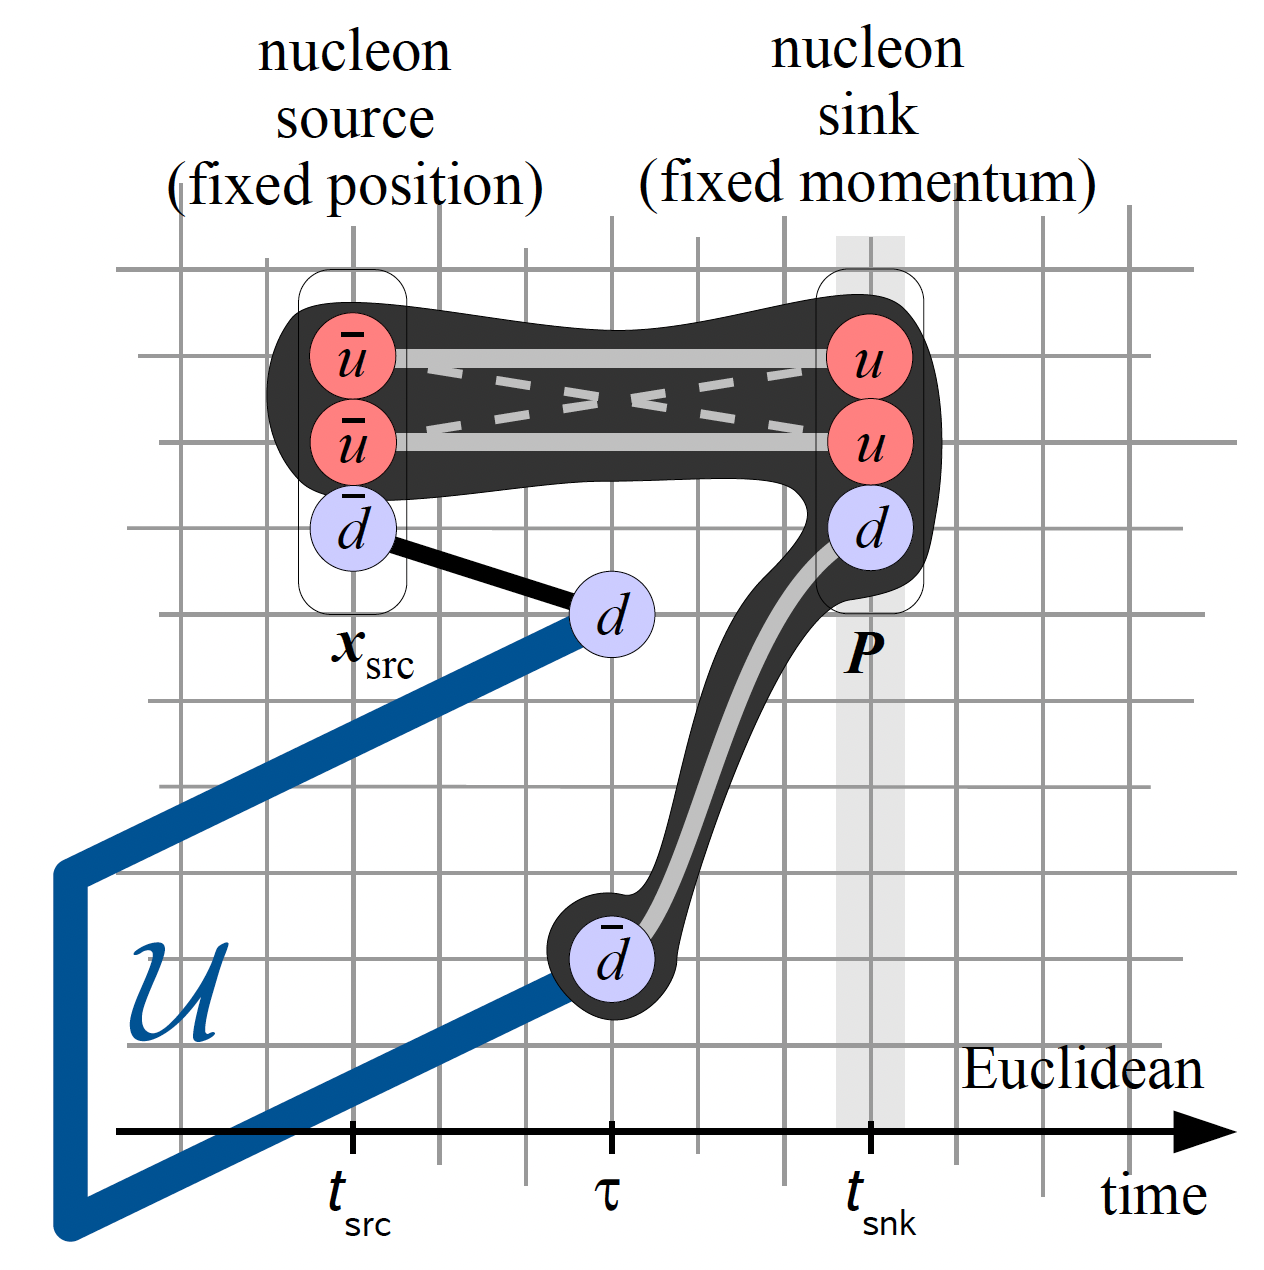
\includegraphics[scale=0.23]{Screenshot 2023-06-14 at 12.38.30 PM.png}
\end{figure}
\begin{itemize}
    \item Evaluate directly ${\widetilde \Phi_\unsub^{[\Gamma]}(\bvec,P,S,\hat \zeta, \mu)}
		\equiv\frac{1}{2}\, \bra{P,S}\ \bar{q}(0)\, \Gamma\ \textcolor{blue}{\Wline{0, \eta v, \eta v + b, b}}\ q(\bvec)\ \ket{P,S}$
   \item Euclidean time: Place entire operator at one time slice, i.e., $b$, $\eta v$ purely spatial.
   \item Extrapolate $\eta\longrightarrow\infty$, $\hat \zeta\longrightarrow\infty$ numerically.
\end{itemize}
\end{frame}

\begin{frame}{Numerical Results}
\begin{figure}
    \centering
    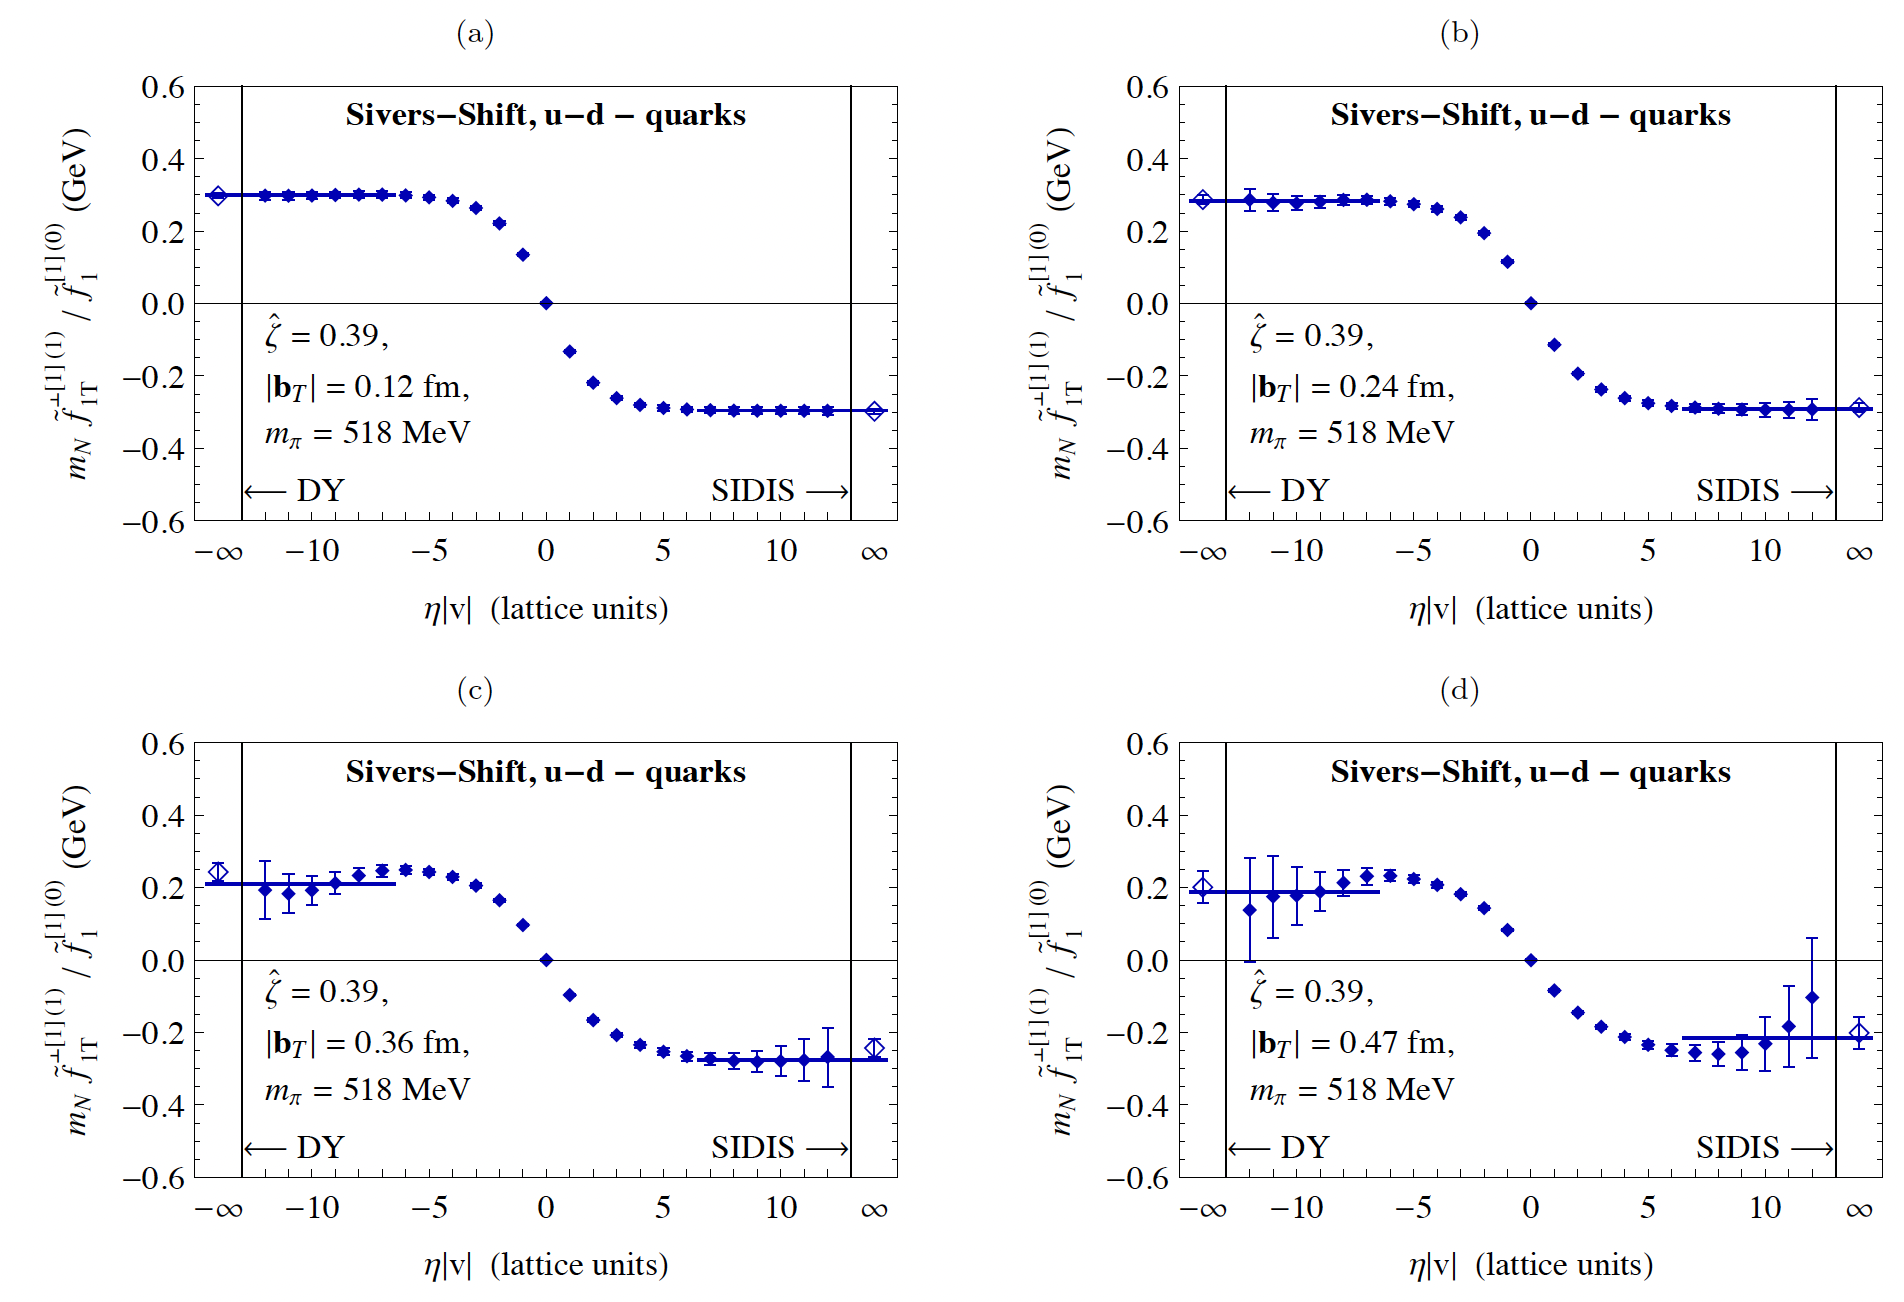
\includegraphics[scale=0.32]{Screenshot 2023-06-14 at 1.01.40 PM.png}
    \caption{Extraction of the generalized Sivers shift on the lattice with $m_\pi= 518$MeV ~\textit{(arXiv:1111.4249v2 [hep-lat])}}
\end{figure}
\end{frame}

\begin{frame}{Numerical Results}
\begin{figure}
    \centering
    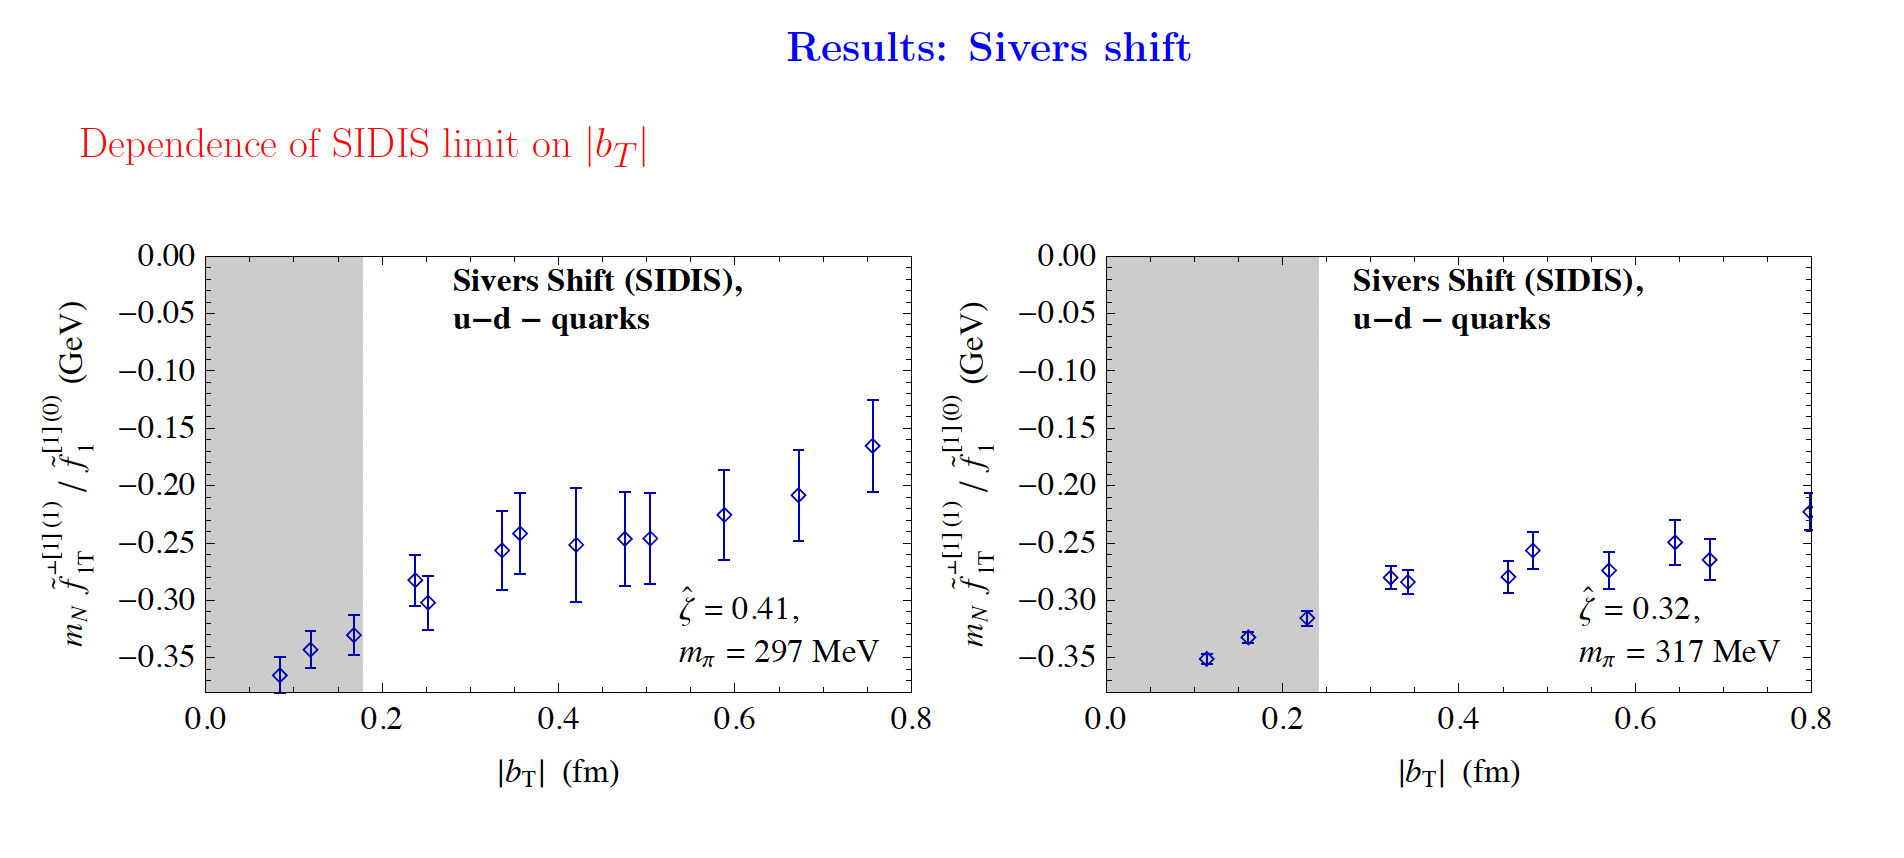
\includegraphics[scale=0.45]{Screenshot 2023-06-14 at 1.06.27 PM.png}
    \caption{Generalized Sivers shift as a function of the quark separation $|\vprp{\bvec}|$ for the SIDIS case ($|\eta v|=\infty$).   ~\textit{arXiv:2301.06118 [hep-lat]}}
\end{figure} 
\end{frame}

\begin{frame}{Numerical Results}
\begin{figure}
    \centering
    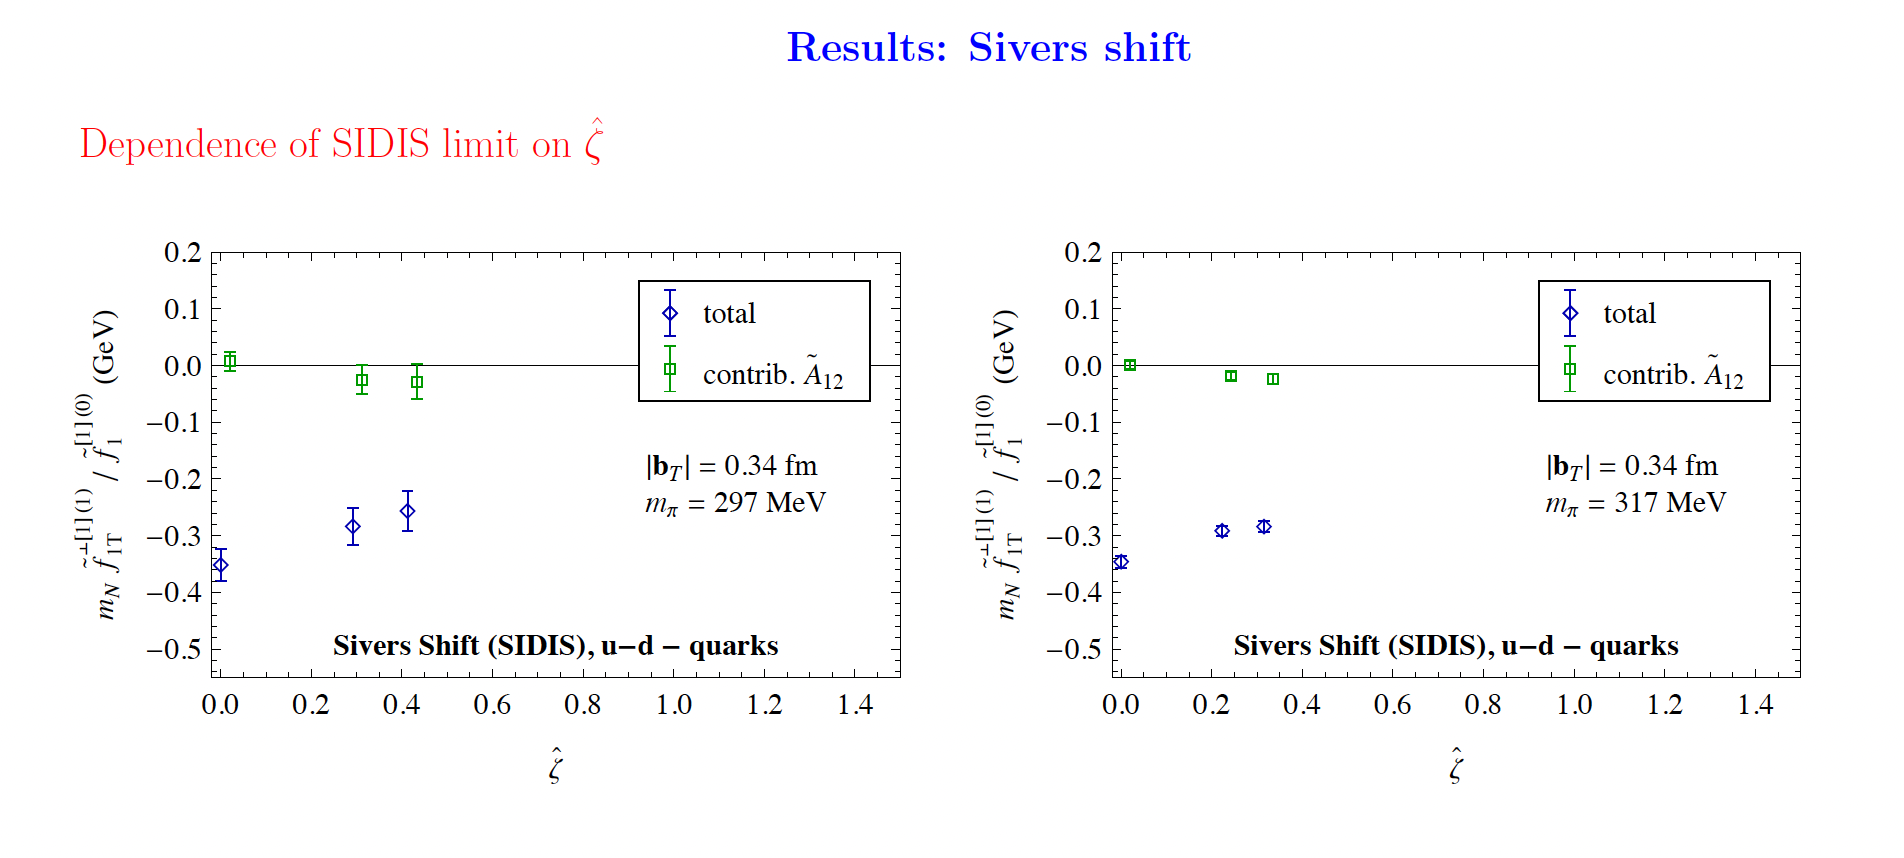
\includegraphics[scale=0.45]{Screenshot 2023-06-14 at 1.06.35 PM.png}
    \caption{we show the $\hat\zeta$-dependence of the generalized Sivers shift, depicting both the full result and the result
obtained with just $\tilde A_{12}$ in the numerator.   ~\textit{arXiv:2301.06118 [hep-lat]}}
\end{figure} 
\end{frame}

\begin{frame}{Few More Numerical Results}
    \begin{itemize}
        \item M.~Engelhardt, \textit{et al.}, PoS \textbf{LATTICE2022}, 103 (2023), [arXiv:2301.06118 [hep-lat]].
        \item B.~Yoon, M.~Engelhardt, R.~Gupta, T.~Bhattacharya, J.~R.~Green, B.~U.~Musch, J.~W.~Negele, A.~V.~Pochinsky, A.~Sch\"afer and S.~N.~Syritsyn, Phys. Rev. D \textbf{96}, no.9, 094508 (2017), [arXiv:1706.03406 [hep-lat]].
        \item M.~Engelhardt, B.~Musch, T.~Bhattacharya, J.~R.~Green, R.~Gupta, P.~H\"agler, S.~Krieg, J.~Negele, A.~Pochinsky and A.~Sch\"afer, \textit{et al.}, EPJ Web Conf. \textbf{112}, 01008 (2016)
        \item M.~Engelhardt, B.~Musch, T.~Bhattacharya, J.~R.~Green, R.~Gupta, P.~Haegler, J.~Negele, A.~Pochinsky, A.~Schafer and S.~Syritsyn, \textit{et al.}, PoS \textbf{QCDEV2015}, 018 (2015)
        \item M.~Engelhardt, B.~Musch, T.~Bhattacharya, R.~Gupta, P.~H\"agler, S.~Krieg, J.~Negele, A.~Pochinsky, S.~Syritsyn and B.~Yoon, PoS \textbf{LATTICE2015}, 117 (2016)
    \end{itemize}
\end{frame}



\begin{frame}{My PhD work: Extension to include the dependence on $x=\frac{k^{+}}{P^{+}}$}
\begin{align}
    \frac{1}{2} \bra{P,S}\ \bar{q}(0)\ \gamma^{+}\ \WlineC{\mathcal{C}_\bvec}\ q(\bvec)\ \ket{P,S}=2P^{+}\left(\textcolor{red}{\tAmp_{2B} }
		+ i \mN \epsilon_{ij} \vect{\bvec}_i \vect{S}_j\, \textcolor{red}{\tAmp_{12B} }\right)
\end{align}
\begin{align}
   \Longrightarrow~ \langle \vect{k}_y \rangle_{TU}(\vprp{\bvec}^2,\textcolor{blue}{x},\zetahat,\eta v \tcdot P) 
	&\ \equiv\ \mN \frac{\tilde f_{1T}^{\perp(1)}(\vprp{\bvec}^2;\zetahat,\ldots,\eta v \tcdot P)}{\tilde f_1^{(0)}(\vprp{\bvec}^2;\zetahat,\ldots,\eta v \tcdot P)}\\
 &=-m_{N} \frac{\int d(b\cdot P)e^{ix(b\cdot P)} \textcolor{red}{\tAmp_{12B}(\bvec^2,\bvec \tcdot P,(\bvec \tcdot P) R(\zetahat^2)/\mN^2,-1/(\mN\zetahat)^2,\eta v \tcdot P)}}{\int d(b\cdot P)e^{ix(b\cdot P)}\textcolor{red}{\tAmp_{2B}(\bvec^2,\bvec \tcdot P,(\bvec \tcdot P) R(\zetahat^2)/\mN^2,-1/(\mN\zetahat)^2,\eta v \tcdot P)}}
\end{align}
\begin{itemize}
    \item The range of accessible $b \cdot P$ is limited:
\end{itemize}
\begin{align}
    \boxed{\textcolor{blue}{\frac{v \tcdot b}{v \tcdot P} = b \tcdot P \frac{R(\zetahat^2)}{\mN^2}\, ,}}
	~~~~~\because\text{($b^{+}=0$ and $v_{T} = \mathbf{P}_{T} = 0$)}\label{eq-lindeprel}
\end{align}
where $R(\zetahat^2) \equiv 1- \sqrt{1 + \hat \zeta^{-2}} = \frac{\mN^2}{v \tcdot P} \frac{v^+}{P^+}$.
\begin{figure}
            \centering
            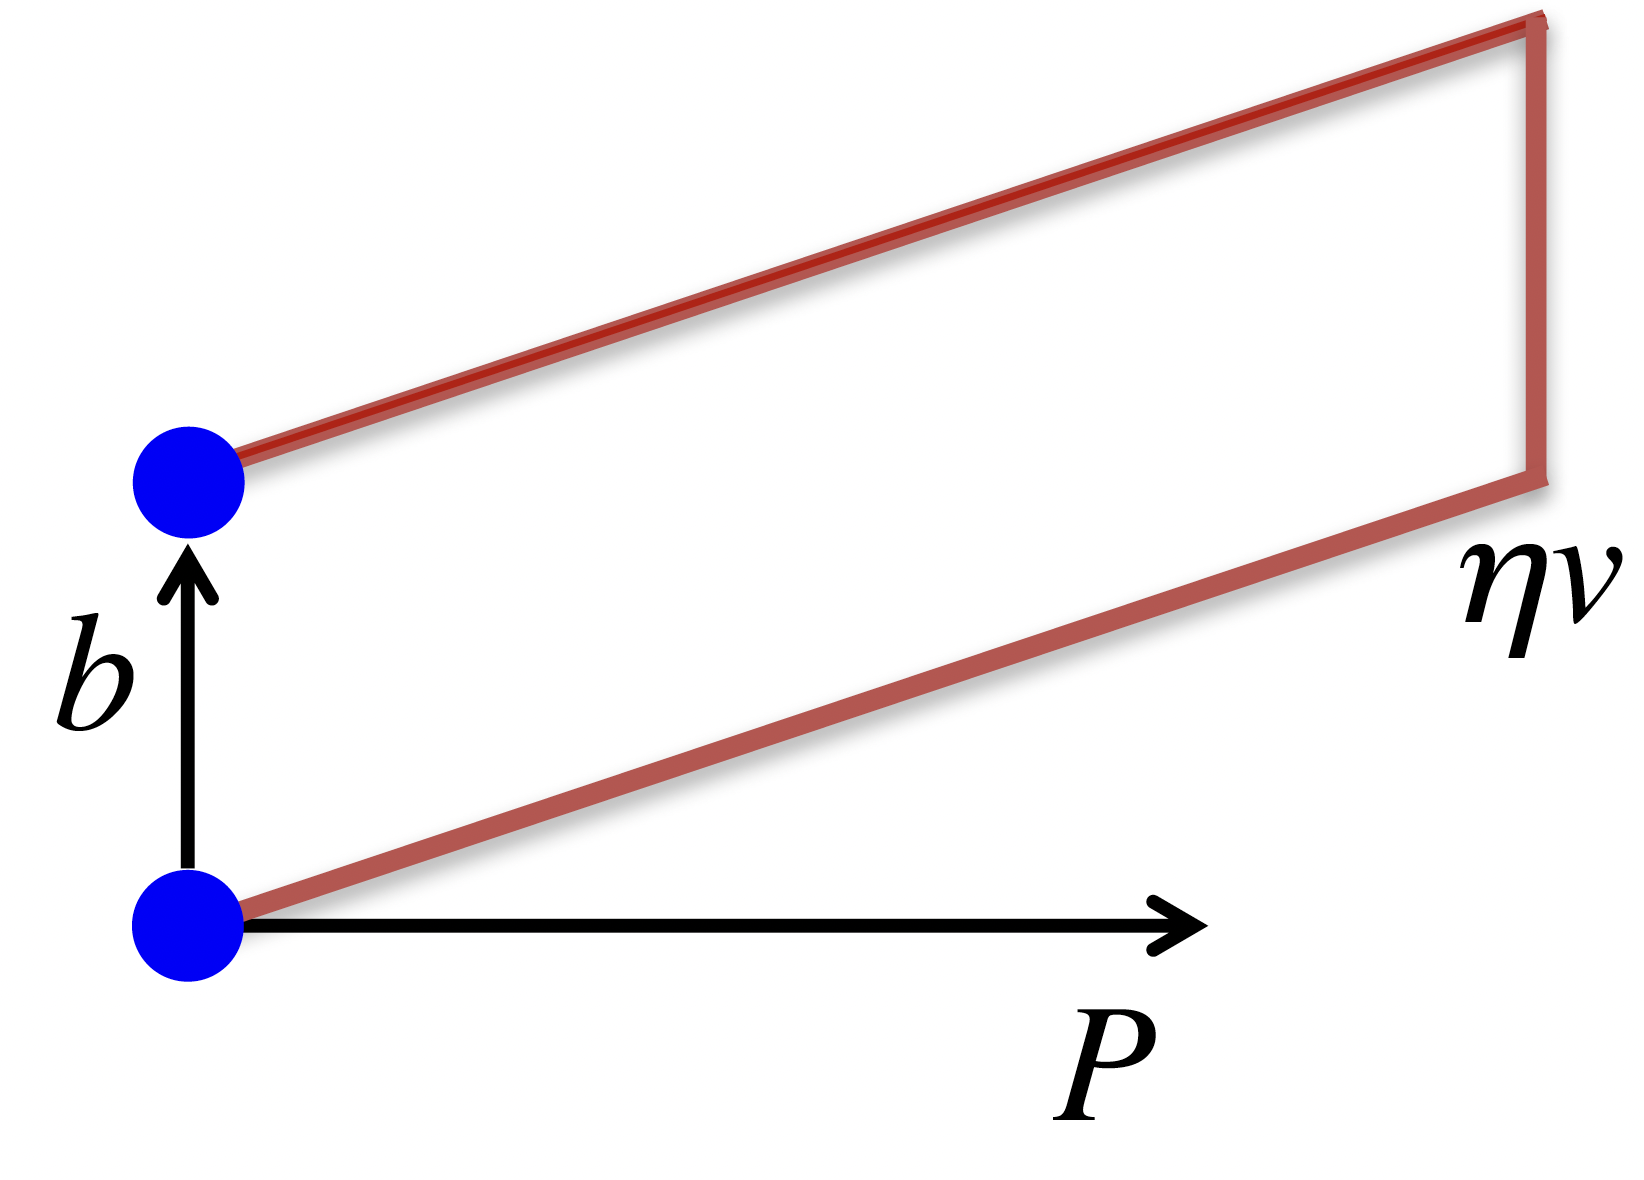
\includegraphics[scale=0.092]{Screenshot 2023-06-14 at 2.24.43 PM.png}
            %\caption{Illustration of the TMD operator with staple-shaped gauge connection}
            \label{fig:enter-label}
        \end{figure}
\end{frame}

\begin{frame}{My PhD work: Extension to include the dependence on $x=\frac{k^{+}}{P^{+}}$}
    \begin{figure}
        \centering
        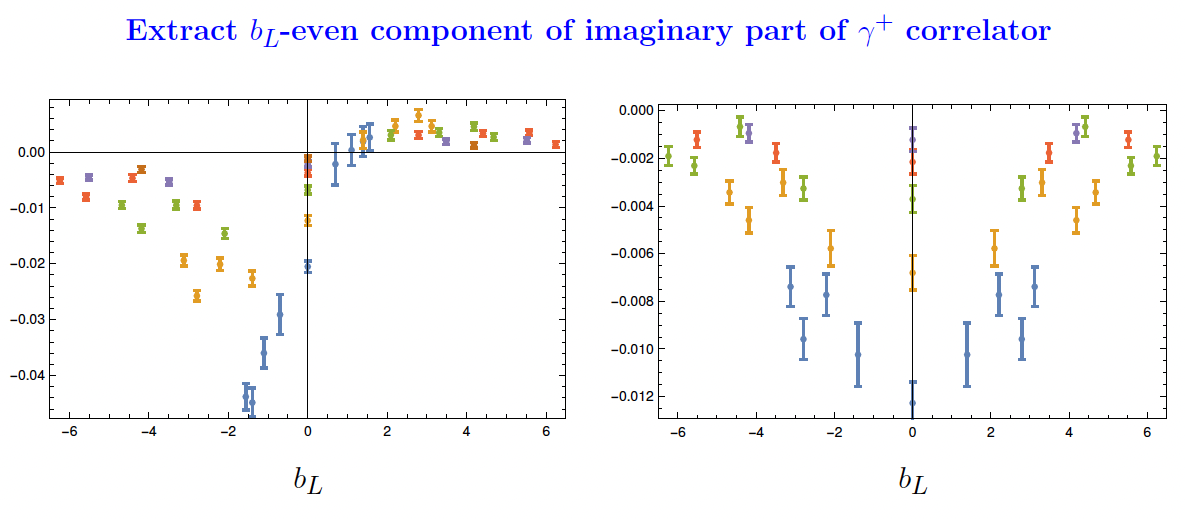
\includegraphics[scale=0.3]{Screenshot 2023-11-08 at 10.47.33 PM.png}
        \caption{\footnote{PDFLattice 2019: M. Engelhardt}        $\left[\frac{1}{2} \bra{P,S}\ \bar{q}(0)\ \gamma^{+}\ \WlineC{\mathcal{C}_\bvec}\ q(\bvec)\ \ket{P,S}=2P^{+}\left(\textcolor{red}{\tAmp_{2B} }
		+ i \mN \epsilon_{ij} \vect{\bvec}_i \vect{S}_j\, \textcolor{red}{\tAmp_{12B} }\right)\right]$}
        \label{fig:enter-label}
    \end{figure}
\end{frame}

\begin{frame}{My PhD work: Extension to include the dependence on $x=\frac{k^{+}}{P^{+}}$}
    \begin{figure}
        \centering
        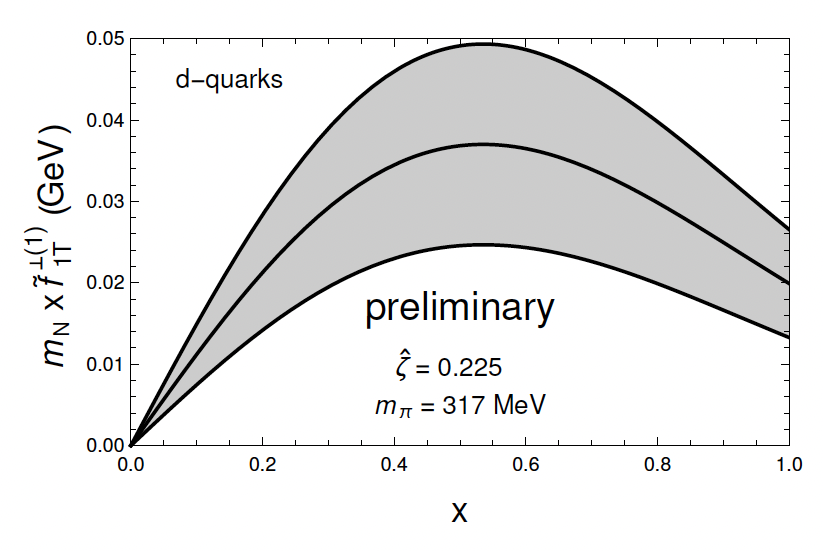
\includegraphics[scale=0.3]{Screenshot 2023-11-08 at 3.01.57 PM.png}
        \caption{Nucleon SIDIS $d$-quark generalized Sivers shift as a function of momentum fraction $x$, multiplied by $x$ \footnote{"TMD Handbook."	arXiv:2304.03302 [hep-ph].}\footnote{M. Engelhardt, J. R. Green, S. Krieg, S. Meinel, J. Negele, A. Pochinsky et al., to be published}}
        \label{fig:enter-label}
    \end{figure}
\end{frame}
\begin{frame}{Conclusions}
    \begin{itemize}
        \item It is feasible to obtain the
$x$-dependence of TMD ratios: \textbf{Sivers shift}
        \item Inspite of constraints  $\frac{v \tcdot b}{v \tcdot P} = b \tcdot P \frac{R(\zetahat^2)}{\mN^2}$, it is possible to improve the analysis
    \end{itemize}
\end{frame}
\end{document}